%-------------------------------------------------------------------------------------
%	PACKAGES AND OTHER DOCUMENT CONFIGURATIONS
%-------------------------------------------------------------------------------------

\documentclass{article}

    \usepackage{fancyhdr} % Required for custom headers
    \usepackage{lastpage} % Required to determine the last page for the footer
    \usepackage{extramarks} % Required for headers and footers
    \usepackage[usenames,dvipsnames]{color} % Required for custom colors
    \usepackage{graphicx} % Required to insert images
    \usepackage{listings} % Required for insertion of code
    \usepackage{courier} % Required for the courier font
    \usepackage{tabularx}
    \usepackage{longtable}
    \usepackage{caption}
    \usepackage{subcaption}
    \usepackage{amsmath}
    \usepackage{mathtools}
    \usepackage{url}
    \usepackage{hyperref}
    \usepackage{amssymb}
    \hypersetup{
        colorlinks=true,
        linkcolor=blue,
        filecolor=magenta,
        urlcolor=blue,
        citecolor=red,
    }
    \captionsetup{
        singlelinecheck=false, 
        format=hang, 
        justification=raggedright, 
        font=footnotesize, 
        % labelsep=space
    }
    \renewcommand{\labelenumii}{\theenumii}
    \renewcommand{\theenumii}{\theenumi.\arabic{enumii}.}
    
    % Margins
    \topmargin=-0.45in
    \evensidemargin=0in
    \oddsidemargin=0in
    \textwidth=6.5in
    \textheight=9.0in
    \headsep=0.25in
    
    \linespread{1.1} % Line spacing
    
    % Set up the header and footer
    \pagestyle{fancy}
    \lhead{\AuthorName} % Top left header
    \chead{\Title} % Top center head
    \rhead{\firstxmark} % Top right header
    \lfoot{\lastxmark} % Bottom left footer
    \cfoot{} % Bottom center footer
    \rfoot{Page\ \thepage\ of\ \pageref*{LastPage}} % Bottom right footer
    \renewcommand\headrulewidth{0.4pt} % Size of the header rule
    \renewcommand\footrulewidth{0.4pt} % Size of the footer rule
    
    \setlength\parindent{0pt} % Removes all indentation from paragraphs
    
    %---------------------------------------------------------------------------------
    %	CODE INCLUSION CONFIGURATION
    %---------------------------------------------------------------------------------
    
    \definecolor{MyDarkGreen}{rgb}{0.0,0.4,0.0} % This is the color used for comments
    \lstloadlanguages{Perl} % Load Perl syntax for listings, for a list of other languages supported see: ftp://ftp.tex.ac.uk/tex-archive/macros/latex/contrib/listings/listings.pdf
    \lstset{language=Perl, % Use Perl in this example
            frame=single, % Single frame around code
            basicstyle=\small\ttfamily, % Use small true type font
            keywordstyle=[1]\color{Blue}\bf, % Perl functions bold and blue
            keywordstyle=[2]\color{Purple}, % Perl function arguments purple
            keywordstyle=[3]\color{Blue}\underbar, % Custom functions underlined and blue
            identifierstyle=, % Nothing special about identifiers
            commentstyle=\usefont{T1}{pcr}{m}{sl}\color{MyDarkGreen}\small, % Comments small dark green courier font
            stringstyle=\color{Purple}, % Strings are purple
            showstringspaces=false, % Don't put marks in string spaces
            tabsize=5, % 5 spaces per tab
            %
            % Put standard Perl functions not included in the default language here
            morekeywords={rand},
            %
            % Put Perl function parameters here
            morekeywords=[2]{on, off, interp},
            %
            % Put user defined functions here
            morekeywords=[3]{test},
               %
            morecomment=[l][\color{Blue}]{...}, % Line continuation (...) like blue comment
            numbers=left, % Line numbers on left
            firstnumber=1, % Line numbers start with line 1
            numberstyle=\tiny\color{Blue}, % Line numbers are blue and small
            stepnumber=5 % Line numbers go in steps of 5
    }
    
    % Creates a new command to include a perl script, the first parameter is the filename of the script (without .pl), the second parameter is the caption
    \newcommand{\perlscript}[2]{
    \begin{itemize}
    \item[]\lstinputlisting[caption=#2,label=#1]{#1.pl}
    \end{itemize}
    }
    
    %---------------------------------------------------------------------------------
    %	DOCUMENT STRUCTURE COMMANDS
    %	Skip this unless you know what you're doing
    %---------------------------------------------------------------------------------
    
    % Header and footer for when a page split occurs within a problem environment
    \newcommand{\enterProblemHeader}[1]{
    % \nobreak\extramarks{#1}{#1 continued on next page\ldots}\nobreak
    % \nobreak\extramarks{#1 (continued)}{#1 continued on next page\ldots}\nobreak
    }
    
    % Header and footer for when a page split occurs between problem environments
    \newcommand{\exitProblemHeader}[1]{
    % \nobreak\extramarks{#1 (continued)}{#1 continued on next page\ldots}\nobreak
    % \nobreak\extramarks{#1}{}\nobreak
    }
    
    % \setcounter{secnumdepth}{0} % Removes default section numbers
    \newcounter{homeworkProblemCounter} % Creates a counter to keep track of the number of problems
    
    \newcommand{\homeworkProblemName}{}
    \newenvironment{homeworkProblem}[1][Problem \arabic{homeworkProblemCounter}]{ % Makes a new environment called homeworkProblem which takes 1 argument (custom name) but the default is "Problem #"
    \stepcounter{homeworkProblemCounter} % Increase counter for number of problems
    \renewcommand{\homeworkProblemName}{#1} % Assign \homeworkProblemName the name of the problem
    \section{\homeworkProblemName} % Make a section in the document with the custom problem count
    \enterProblemHeader{\homeworkProblemName} % Header and footer within the environment
    }{
    \exitProblemHeader{\homeworkProblemName} % Header and footer after the environment
    }
    
    \newcommand{\problemAnswer}[1]{ % Defines the problem answer command with the content as the only argument
    \noindent\framebox[\columnwidth][c]{\begin{minipage}{0.98\columnwidth}#1\end{minipage}} % Makes the box around the problem answer and puts the content inside
    }
    
    \newcommand{\homeworkSectionName}{}
    \newenvironment{homeworkSection}[1]{ % New environment for sections within homework problems, takes 1 argument - the name of the section
    \renewcommand{\homeworkSectionName}{#1} % Assign \homeworkSectionName to the name of the section from the environment argument
    \subsection{\homeworkSectionName} % Make a subsection with the custom name of the subsection
    \enterProblemHeader{\homeworkProblemName\ [\homeworkSectionName]} % Header and footer within the environment
    }{
    \enterProblemHeader{\homeworkProblemName} % Header and footer after the environment
    }
    
    %---------------------------------------------------------------------------------
    %	CUSTOM MATH COMMANDS
    %---------------------------------------------------------------------------------
    \newcommand{\erf}{\mathrm{erf}}
    \newcommand{\N}{\mathcal{N}}
    \newcommand{\A}{\hat{A}}
    \newcommand{\MU}{\hat{\mu}}
    \newcommand{\SIGMA}{\hat{\sigma}}
    
    %---------------------------------------------------------------------------------
    %	NAME AND CLASS SECTION
    %---------------------------------------------------------------------------------
    
    \newcommand{\Title}{Cyton Solver}
    \newcommand{\InstituteName}{Hodgkin Lab \\ Walter and Eliza Hall Institute of Medical Research}
    \newcommand{\AuthorName}{HoChan, Cheon} % Your name
    %---------------------------------------------------------------------------------
    %	TITLE PAGE
    %---------------------------------------------------------------------------------
    
    \title{
        \vspace{2in}
        \textmd{\textbf{\Title}} \\
        \vspace{0.1in}
        % \normalsize\vspace{0.1in}\small{\today}\\
        
\includegraphics{./img/WEHI_logo}
        \centering
        \\
        \vspace{-0.1in}
        \vspace{0.1in}\large{\textit{\InstituteName}}
        \vspace{3in}
    }
    
    \author{\textbf{\AuthorName} \\ \href{mailto:cheon.h@wehi.edu.au}{cheon.h@wehi.edu.au}}
    \date{\today} % Insert date here if you want it to appear below your name
    
    %---------------------------------------------------------------------------------
    \setlength{\parindent}{1em}
    
    \begin{document}
    
    \maketitle
    
    %---------------------------------------------------------------------------------
    %	TABLE OF CONTENTS
    %---------------------------------------------------------------------------------
    
    %\setcounter{tocdepth}{1} % Uncomment this line if you don't want subsections listed in the ToC
    
    \newpage
    \tableofcontents
    \newpage
    
    %---------------------------------------------------------------------------------
    %	SECTION 1 : Release notes
    %---------------------------------------------------------------------------------
    \begin{homeworkProblem}[Release Notes]
        \begin{itemize}
            \item v1.1.4b
            \begin{itemize}
                \item[+] added new optimisation algorithm, \href{http://infinity77.net/global_optimization/ampgo.html}{AMPGO} (Adaptive Memory Programming for Global Optimisation)
                \item[+] issue warning message for importing HL-SEP-2016 data format
                \item[+] (under-dev) still fixing an issue with spawning thread for bootstrapping 
            \end{itemize}

            \item v1.1.3b
            \begin{itemize}
                \item[+] fit to total cell
                \item[+] added Model end time in \textit{Model Settings} \\ NB: It only changes last time point number in default harvested time list. A better way of doing this is to let an end-user to modify harvested times directly. More to come...
                \item[+] fixed an issue with Windows OS scaling 
            \end{itemize}

            \item v1.1.2b
            \begin{itemize}
                \item[+] added support for modifying initial cell number
                \item[+] (testing) added support for HighDPI monitor, especially for Windows scaling
                \item[+] (under-dev) added backbone strcutrue for bootstrap method for any given \% confidence interval  
            \end{itemize}

            \item v1.1.1b
            \begin{itemize}
                \item[+] completed basic layout and feature for \textit{Compare} tab
            \end{itemize}

            \item v1.1.0b
            \begin{itemize}
                \item[+] overhaul code structure. Optimised throughput performance, simplified variable names for future developers, and better overall code logic
                \item[--] removed batch fitting (only left with placeholders)
                \item[+] added two new place holder tabs 1.\textit{About} (for introduction page to Cyton Soler) 2. \textit{Compare} (for comparing distributions from saved parameters)
            \end{itemize}
            
            \item v1.0.4b
            \begin{itemize}
                \item[+] add queuing conditions in fit process (called batch process) -> automatically save fitted parameters and export plots
            \end{itemize}

            \item v1.0.3b
            \begin{itemize}
                \item[+] import legacy data format
                \item[+] fixed an issue with legacy data format with asymmetric time points
                \item[+] changed \textit{Export Plot} output folder name from placeholder text to condition name (adding suffix wiht 4 leading zeros to avoid overwriting)
                \item[+] replaced toolbar (list of icons) to dropdown menubars (File \& Tools)   
            \end{itemize}

            \item v1.0.2b
            \begin{itemize}
                \item[+] added Data Free mode for all states of the program.
            \end{itemize}
            \item v1.0.1b
            \begin{itemize}
                \item[+] \textit{Export Plot} button will generate plot\_table\_view.xlsx for easier plotting in Prism
            \end{itemize}
        \end{itemize}
    \end{homeworkProblem}

    %---------------------------------------------------------------------------------
    %	SECTION 2 : The program
    %---------------------------------------------------------------------------------
    \clearpage
    \begin{homeworkProblem}[Cyton Solver]
        The program is far from being perfect nor complete as more features were requested at every step of development leaps and discussions. I aimed to design it as general as possible to cover the most likely use case of the Cyton model, and at the same time, create an intuitive interfaces so people can immediately grasp the functions behind them. However, I realised that condensing too much information sometimes sets more drawbacks than its potential benefits. So here I will layout complete manual of the Cyton Solver, not only for the features implemented in the program but the actual \textit{mathe-magics}. 
        

        This guide is generally for internal use in Hodgkin lab, but you can send me an \href{mailto:cheon.h@wehi.edu.au}{email} to get downloadable link. For those who have an access to the shared folder on WEHI server, it is located in (as of 21-Dec-2018), 

        \begin{center}  
            \verb+\\FS_ALL\Hodgkin_Share\software\cyton-solver+
        \end{center}

        One last note... the technical part of the software was sorely developed by myself, so even though I tried my best to capture as much common errors as possible, it is still prone to crashes without any obvious reasons or guidelines. It might be due to importing an incorrect data format, or lack of system memory as I did not particularly design it memory efficient. If you do find unusual crashes/errors, please feel free to give me any feedback via email. As for future developer(s) who wish to build better program based on this, I highly recommend to spend half of efforts to design systematic test suite (e.g. unit test) from the beginning.
        
        %-----------------------------------------------------------------------------
        %	SECTION 2.1 : Quick Start
        %-----------------------------------------------------------------------------
        \subsection{Quick Start}
            \subsubsection{For modellers}
            \begin{enumerate}
                \item Unzip [CytonSolver v1.1.3b.zip]. If you are on the server, choose one that appropriate for your OS.
                \begin{enumerate}
                    \item (MAC) Simply double click [\textit{CytonSolver.app}] application
                    \item (WIN) Navigate to ``CytonSolver'' folder $\rightarrow$ scroll down to find [\textit{CytonSolver.exe}] (do NOT move this file! Make a shortcut to the desktop if you wish)
                \end{enumerate}
                \item[$>$] IMPORTANT!! At this point please have a look at the provided example data files, and familiarise yourself with the data format.
                \item Import an example data file
                \begin{enumerate}
                    \item You can directly import the file by ``File $\rightarrow$ Open...'' or Ctrl+O/CMD+O. However, using this data format is NOT recommended.
                    \item Instead please utilise [\textit{Cohort Explorer v2018.05.09}] by drag \& drop data file into it.
                    \item Once [\textit{Cohort Explorer}] finishes its analysis, it generates a new folder (same name as the input data file) located in the same folder as the input. Note that this software will NOT overwrite any existing folders.
                    \item Find an output excel file, which is usually named after the input data file with suffix \_4prism, e.g. FILE\_NAME\_4prism.xlsx.
                    \item Import FILE\_NAME\_4prism.xlsx from [\textit{CytonSolver}] (step 2.1)
                \end{enumerate}  
                \item[$>$] NB: Yes, you may stop at step 2.1, and not bother to run [\textit{Cohort Explorer}] from the beginning. However, it is always a good practice to check your data before getting into the modelling. Perhaps it will give you an insight on what to expect from the model or find outlier(s). Take the entire step 2 as an analysis pipeline so that one can get a bigger picture to what data is about to reveal.
            \end{enumerate}

            \subsubsection{For developers}
            \begin{itemize}
                \item \textit{CytonSolver} is written in \href{https://www.python.org/downloads/release/python-365/}{Python v3.6.5}. It is highly recommended to create a virtual environment to isolate the project from your default global python settings and libraries.

                Before you begin coding, set the project root to be one path ABOVE ``/src'' folder so that your root must contain ``/img'', ``/src'', and any other output folders you may wish to add.
    
                All of dependencies are listed in \textit{requirements.txt}, and you will soon realise that this needs constant updates and testings as package devlopers release new version of them at different time frame. You can invoke following command to install pre-defined versions of the packages.
                \begin{lstlisting}
                    $ pip install -r requirements.txt
                \end{lstlisting}
                Core algorithms are written in \href{https://cython.org/#documentation}{Cython} language to reduce computational costs, thus you need to compile these scripts to OS specific. It is basically C-extensions for python that converts interpret language to machine compiled instructions. I was able to achieve a little over 100x performance gain compared to a pure python script, so I highly recommend to use it unless you have better alternatives. The target scripsts are located in,
                \begin{lstlisting}
                    $ src/workbench/cyton1/c1_model.pyx
                    $ src/workbench/cyton15/c15_model.pyx
                \end{lstlisting}
                and use following command to compile,
                \begin{lstlisting}
                    $ python CythonSetup.py build_ext --inplace
                \end{lstlisting}
                I would assume that you probably encounter some issues at this point, but be patient and read error outputs. They are generally quite useful, and it is similar to C/C++ standard error output style. It is also possible that even though the scripts are succesfully compiled, the executable files are not functioning properly or straight refused to launch. To debug this, there is an identically bundled app with console logger, and by launching it, you should be able to locate where it causes an error within the entire program.

                Succesfully compiling the Cython scripts will create shared library objects, which can be accessed by the usual pythonic way (e.g. \verb+from example import example_class+). Now you should find no problem invoking main entry script to initiate the program.
                \begin{lstlisting}
                    $ python /src/gui/main_cs.py
                \end{lstlisting}
                
                \item Building a single exceutible application requires \href{https://www.pyinstaller.org/}{PyInstaller} library. Note that it is highly susceptible to versions of PyInstaller, matplotlib, and Python interpreter imported in the bundling process, and as such, please do not update the packages without testing them. The support usually comes after new release from the developers.
                
                In order to build MAC version of the program, run
                \begin{lstlisting}[language=bash]
        $ python -m PyInstaller --clean -y -w -F MAC-cyton-solver.spec
                \end{lstlisting}
                \textit{MAC-cyton-solver.spec} is the specification file that I wrote to define and wrap external resources (e.g. images) and dependencies. It also locates the main entry point of the program, and analyses all the modules and grab them into a single file.

                In order to build WINDOWS version of the program, run
                \begin{lstlisting}[language=bash]
        $ python -m PyInstaller --clean -y -w -F WIN-cyton-solver.spec
                \end{lstlisting}
                This will result in slightly different style than that of MAC version. It somehow does not create a clean app like MAC, but it simply copies all libraries in a single folder with the executable, \textit{CytonSolver.exe}. It is required to leave those files at where they are in order for the program to locate them properly, so do not arbitrarly rename or move them.
            \end{itemize}
            
        %-----------------------------------------------------------------------------
        %	SECTION 2.2 : Cyton Solver Overview
        %-----------------------------------------------------------------------------
        \subsection{Overview}
        \begin{figure}[ht]
            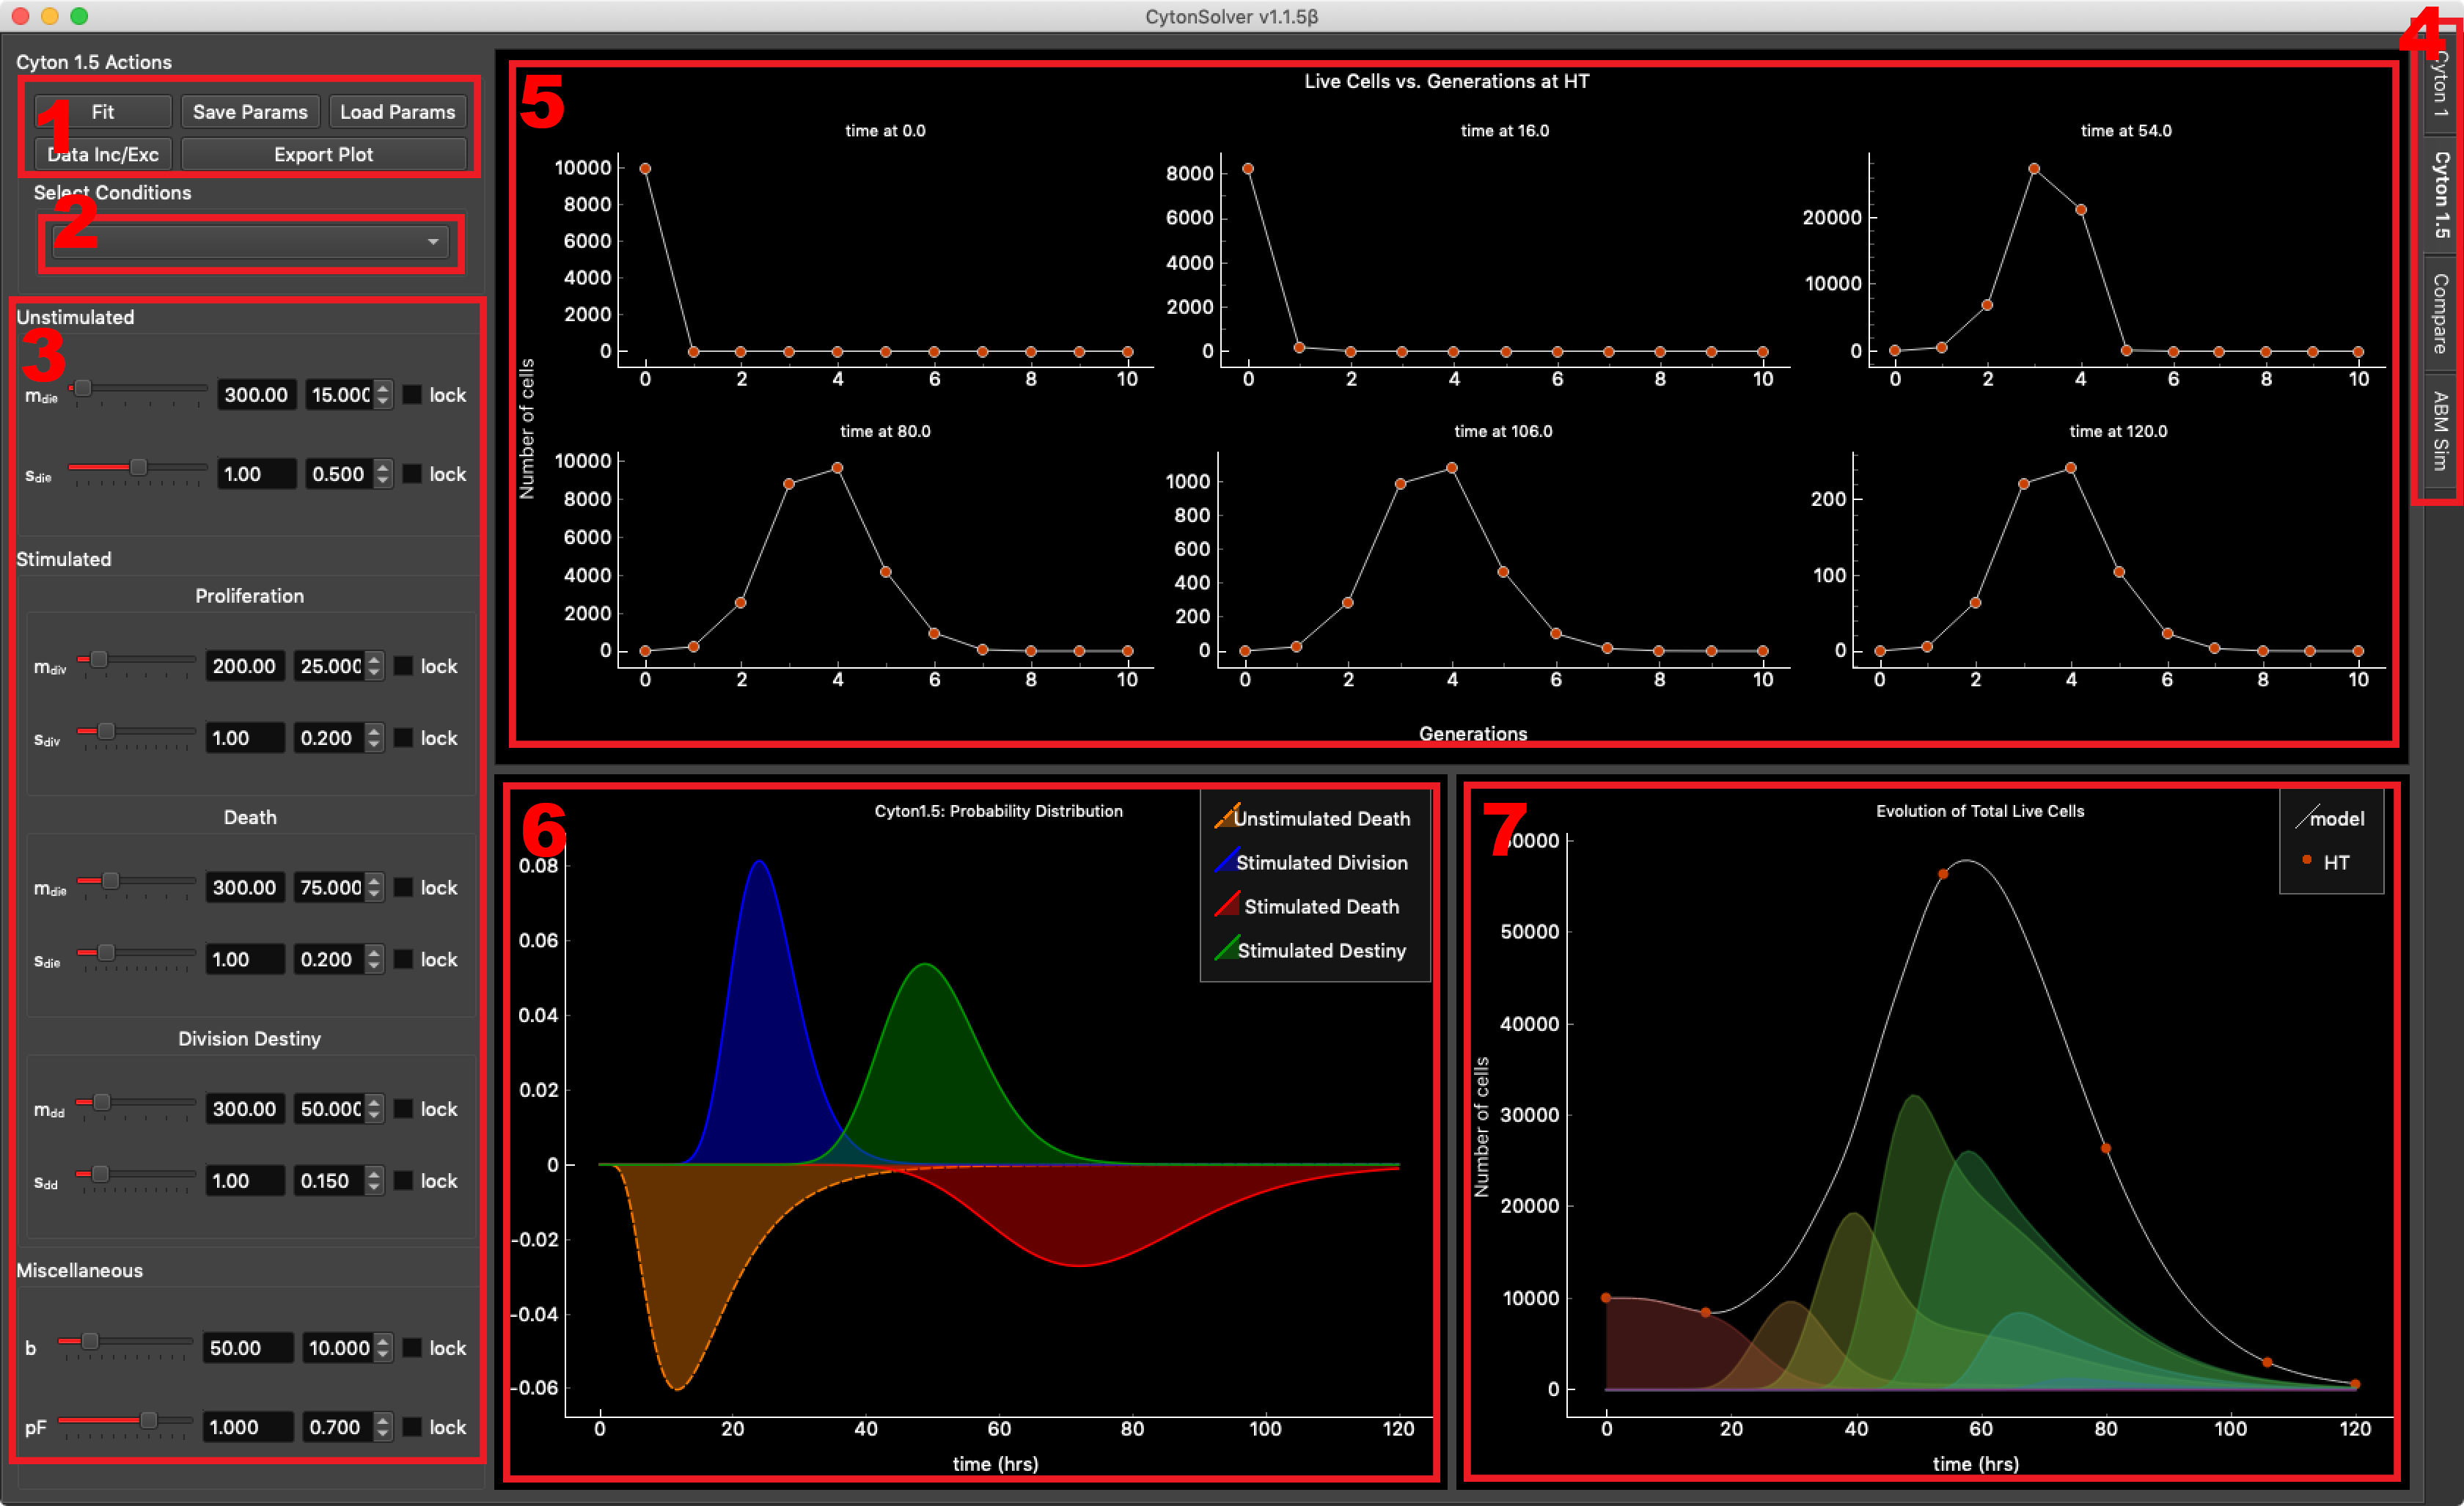
\includegraphics[scale=0.27]{./img/CytonSolver_v115b}
            \centering
            \caption{Cyton Solver main window}
            \label{fig:Cyton Solver}
        \end{figure}
        \begin{longtable}{|c||m{42em}|}
            \hline
            1 & Model specific action buttons: 
            \begin{itemize}
                \item Initiate curve fitting to data (default: disabled). Enabled when data is imported.
                \item Save and load parameters. System creates an excel file at default location (data file directory). Load parameter requires at least one entry in the excel file.
                \item Data inclusion \& exclusion for fitting. Excluded data points are ignored from optimisation.
                \item Export current plots in the main window, and hidden information (e.g. number of dead cells) at default location (data file directory). Table view of the plots are exported as excel file to plot in Prism or other plotting softwares.
            \end{itemize} \\
            \hline
            2 & Select experiment condition. Enabled when data is imported. Values of parameters are shared across all conditions. \\
            \hline
            3 & Parameter control centre (from left to right: slider, maximum value, current value, and lock parameter from fitting). Locked parameters are ignored during optimisation. \\
            \hline
            4 & Mode switch:
            \begin{itemize}
                \item Cyton 1
                \item Cyton 1.5 (default)
                \item Compare. Quick tool to compare probability distributions for Cyton1.5 (requires saved parameters).
                \item Agent-based simulation
            \end{itemize} \\
            \hline
            \hline
            5 & Number of live cells at harvested time points. Default harvested time points are 0, 16, 54, 80, 106, 120 hours. It automatically detects harvested time points in a data file, and adjusts the size of the plots accordingly. \\
            \hline
            6 & Current probability distribution setup (default: Lognormal). Gaussian (normal) distribution is available in Model Settings (ctrl+M / cmd+M). \\
            \hline
            7 & Total live cells as a function of time. Color blocks are live cell numbers at each generation (default: 10). \\
            \hline
        \end{longtable}
    \end{homeworkProblem}

    %---------------------------------------------------------------------------------
    %	SECTION 3 : Program Features
    %---------------------------------------------------------------------------------
    \newpage
    \begin{homeworkProblem}[Program Features]

        %-----------------------------------------------------------------------------
        %	SECTION 3.1 : Note on Cyton 1
        %-----------------------------------------------------------------------------
        \subsection{Note on Cyton 1}
        This version of Cyton model was originally developed by Hawins et al. \cite{2007Hawkins} in Java language. Detailed algorithm and theory can be found in the supplementary material of the paper. The program is well optimised, and more importantly, is compiled for faster performance. If you are after Cyton 1 modelling, I recommend using this particular software rather than the one that provided in Cyton Solver.

        \begin{figure}[ht]
            \includegraphics[scale=0.18]{./img/2007CytonCalculator.png}
            \centering
            \caption{Cyton Calculator 2007}
            \label{fig:Cyton Calculator 2007}
        \end{figure}
        I ported the exact algorithm from Java to Python for backward compatibility without any python specific optimisation. Hence, it is notably \textit{slower} than the original software; it is a sad consequence of implementing in Python. As building Cyton 1 was not my primary focus, most of buttons in the interface are placeholders that might be implemented in the future. In fact, the interface is exactly equivalent to that of Cyton 1.5, except that the most of features are implemented for newer Cyton model.

        %-----------------------------------------------------------------------------
        %	SECTION 3.2 : Optimisation
        %-----------------------------------------------------------------------------
        \subsection{Optimisation}
        The program offers three different optimisation algorithms.
        \begin{enumerate}
            \item Levenberg-Marquardt (LM) \cite{1944Levenberg}, \cite{1963Marquardt}, \cite{Croeze}
            \item Differential Evolution (DE) \cite{1997StornPrice}
            \item Adaptive Memory Programming for Global Optimisation (AMPGO) \cite{2010Lasdon}
        \end{enumerate}
        \begin{figure}[h]
            \includegraphics[scale=0.5]{./img/fitting.png}
            \centering
            \caption{Importing data file will activate \textbf{Fit} button on upper left corner of Cyton Solver, which brings up a pop up window for user to choose choose various algorithms and options associated with it.}
            \label{fig:fitting_procedure}
        \end{figure}
        LM algorithm is popular for its fast performance and relatively robust\footnote{Terms like ``robust'' or ``well'' fitted curve might sound qualitative and highly subjective. Remember that we can always quantify the optimisation results by computing residual sum of squares (RSS) between data and model predictions. We should also admit that RSS is not the only measure of goodness of fits, and usually served as an indication, \textit{not} the absolute goodness.} optimisation outcomes. Generally for models with lower degrees of freedom perform resonably well. However, LM is known to be susceptible with initial values of parameters such that it is a common practice to provide educated guesses, or to initiate with randomised population of parameter sets. Since Cyton 1.5 requires ten parameters, which inevitably forms a non-linear behaviour, it is arguable that LM method is not ideal to find the true optimal point in such vast parameter space. I suggest to thoroughly investigate the data via cohort analysis, and then use that knowledge in conjunction with LM method. Another important aspect is that LM method requires a differentiable (i.e. continuous \& smooth) function everywhere in real-valued space. Our current Cyton 1.5 model suffers discontinuity with respect to subsequent division time (denoted as $b$ in the program), thus, the algorithm fails to update corresponding parameter. If you wish to optimise \textit{with} subsequent division time, please consider using other algorithms.

        To overcome aformentioned problems, I implemented global optimisation algorithms, DE and AMPGO\footnote{I have to admit that I do not know much about how AMPGO works, and I simply added this algorithm as it was latest feature added on \href{https://lmfit.github.io/lmfit-py/}{LMFIT} package. There are many standard benchmark tests available online that I thought it was worth give a chance for Cyton Solver.}. DE method is inspired by evolutionary processes\footnote{Particle swarm optimisation algorithm is similar alternative based on the same principle.} found in various biological systems. It initially generates a random population of parameters, and stochastically updating/mutating the groups based on the best ranking species. Given that it involves heavy randomisation in process and heuristically search for the most optimal pathway, it does \textit{not} require the objective function to be differentiable, however, it is computationally expensive process.

        As you can see from Figure (\ref{fig:fitting_procedure}), each algorithm has its own specific options that users can choose. By default, I have set all three algorithms to have large maximum iteration number in order to avoid premature termination. The other options are small number criteria ($\epsilon$) that allow the algorithm to terminate if and only if the norm of $n$-th and ($n-1$)th parameter vector is smaller than the $\epsilon$. I found that these numbers do not neccessarily make algorithm accurate nor converge to the solution, so I recommend to use defaults for good balance between computation time and reasonable accuracy. The detailed information about the options are available in Scipy website.

        Lastly, an extra layer of setting, on top of the algorithm, is provided in order to automate repeatable tasks, obtain confidence interval, or re-direct target data points. First two options (``batch fit'' \& ``CI [Bootstrap]'') were implemented previously but taken out for further improvements; batch fit offers scheduling multiple fitting procedures (for more than one condition), but I quickly discovered that it is difficult to distinguish automatically generated files from other existing ones. Confidence interval (CI) uses standard bootstrapping method to obtain any $p\%$ confidence range on optimised parameter values\footnote{I have technical issue with implementing bootstrapping method without freezing or crashing the entire program. I believe it requires a new class that spawns separate threads than the one from fitting protocol. Note that PyQt5 cannot spawn a sub-thread.}. ``Fit to total cells'' fits to total number of cells instead of each cell number per generation. It is especially useful for long time course data that has no cell numbers per generation profile. This particular feature is fully implemented and tested.

        %-----------------------------------------------------------------------------
        %	SECTION 3.3 : Model Settings
        %-----------------------------------------------------------------------------
        \subsection{Model Settings}
        \begin{figure}[h]
            \centering
            \includegraphics[scale=0.5]{./img/model_settings.png}
            \caption{Model settings window}
            \label{fig:model_settings}
        \end{figure}
        You can specify model settings from ``Tools'' $\rightarrow$ ``Model Settings'' (shortcut: CTRL+O or CMD+O). It contains four categories,
        \begin{enumerate}
            \item Time increment ($\Delta t$) in unit of hours 
            \item Initial cell number at $t = 0$ (not neccessarily from initial time point)
            \item Initial time point ($t_0$, disabled for now) \& end time point ($t_f$)
            \item Types of probability distributions; either Normal or Lognormal
        \end{enumerate}
        In an ideal world with infinite computing power and memory, we can handle Cyton results continuously at any given time with infinite precision without any discontinuity in between. However, it is not the case in reality. Thus, we must ``slice'' given time period (usually defined by initial and final time points) such that the computer is subjected to finite amount of time points. For instance, if we are given that $t_0=0$ and $t_f=24$ with $\Delta t=1$, cell numbers are iteratively computed at $t=0, 1, 2, \dots, 24$ respectively. The program will automatically choose the most optimal time increment upon importing data file\footnote{The program selects from $\Delta t = [0.25, 0.5, 1]$ hours. Note that only certain $\Delta t$ can be chosen because ``sliced'' time points must coincide with harvested times in data file for optimisation.}.

        Sometimes it is useful to be able to control number of starting cells. Current version of Cyton Solver automatically calculates the average total cell number (if you have more than one replicate) of first harvested time point, and use that information to compute rest of cell numbers. Remember that the program always start calculating from $t=0$, \textit{not} initial harvested time point!

        The model determines initial and final time points based on the data file\footnote{Default time points are [0, 16, 54, 80, 106, 120].}. I implemented a method to change final time point but with some caveat; last time point \textit{cannot} be less than the second last time point. For example, if you have harvested time points [0, 24, 48, 72], you can change 72 to any number greater than 48. The plot x-ranges will be updated automatically. Better way of solving this is to let user to add/remove time point slots. In this way, there are more flexibility on changing \textit{all} time points rather than final one. But I leave this to future task.

        Another crucial aspect of the Cyton modelling is to be able to choose different probability distributions, either for mathematical rigorousness or to lessen complication. Cyton Solver offers two commonly known distributions in Hodgkin lab, Gaussian (i.e. Normal) or Lognormal distributions. By default the program selects Lognormal distributions for all parameters, but you can easily swap them by clicking the dropdown menus. Each of them are labeled in a box either for Cyton 1 or Cyton 1.5, and corresponding parameter. In theory, you can construct mixed probability distribution configuration, but it would be much easier to justify if you were to choose consistent probability ``mechanism'' across the model setting.

        %-----------------------------------------------------------------------------
        %	SECTION 3.4 : Parameter Management
        %-----------------------------------------------------------------------------
        \subsection{Parameter Management}
        Cyton solver is designed to handle one experiment condition at a time; it can only display result from one parameter configuration. It was originally developed to handle and plot all conditions in a single figure, but I quickly realised that such method imposes some serious visibility issue for experiment with 10+ conditions.

        Note that parameter values displayed on the left side of the program are shared amongst other conditions. It is adviced to save current values each time you complete the analysis (e.g. after fitting). By clicking \textbf{Save Params}, it will prompt a comment input text box, which can be used to identify specific set of parameters later on.
        \begin{figure}[h]
            \centering
            \includegraphics[scale=0.5]{./img/comment_box.png}
            \caption{Insert comment in the empty area. It can accept any string and numbering format in ASCII.}
            \label{fig:comment_box}
        \end{figure}

        In an event of error, you can check Console Log (CTRL+C or CMD+C) for details. Otherwise, it will print a success message and the location\footnote{By default, it saves in the same location where the input data file is. You can move the file to different location, but the program will create another one if you save another parameter set.} of an Excel file (\verb+DATA_FILE_params.xlsx+) that contains, if any, previously saved parameters. Keep in mind that there are \textit{two} worksheets for each Cyton model.
        \begin{figure}[h]
            \centering
            \includegraphics[scale=0.31]{./img/excel_save_params.png}
            \caption{Automatically generated excel file after saving parameters. Two worksheets are used to distinguish Cyton model. Each row represents one parameter set with time stamp, condition name, and comments. All values are saved in double precision data type.}
            \label{fig:excel_save_params}
        \end{figure}

        You can modify any saved quantities in the excel file, including comments, as long as it retains row \& column structures. You may also move the file to different folder, but it is not recommended as the program requires the file at its default location for loading parameter back into the system.

        Loading parameters is as simple as clicking \textbf{Load Params} next to the save button. It will prompt another window for you to choose saved parameters inside the excel. Choose appropriate one from the dropdown menu, and click Ok to update the plots.
        \begin{figure}[h]
            \centering
            \includegraphics[scale=0.42]{./img/load_params.png}
            \caption{Load saved parameter with preview window}
            \label{fig:load_params}
        \end{figure}

        %-----------------------------------------------------------------------------
        %	SECTION 3.5 : Parameter Comparison Tool
        %-----------------------------------------------------------------------------
        \subsection{Parameter Comparison Tool}
        In many of biological systems and experiments, it is often desired to clearly layout the effects of control variables. It can be titration experiment, one or more cellular signal integration etc. The idea behind this tool is to give an easy and quick option to compare results (i.e. probability distributions) without taking further extra step\footnote{Indeed, you can export plot values indiviually and use Prism or any other preferred scientific software to overlay into a single figure. But this can be very time consuming, especially if you have large dataset.}.

        You can access this tool by navigating to \textbf{Compare} tab located on right side of the program. Unfortunately, it only supports Cyton 1.5 with limited features in terms of manipulating figures. The associated Cyton 1.5 parameters are broken into four panels, and the ranges of plots are initially adjusted automatically with imported data. Note that this tool can only be used when you have saved parameter in your current working directory, so make sure you have few results saved before using this feature.

        \begin{figure}[h]
            \centering
            \includegraphics[scale=0.23]{./img/compare_params.png}
            \caption{Cyton 1.5 parameter comparison tool. From left to right, top to bottm, panels correspond to Unstimulated Death, Time to First Division, Stimulated Death, and Division Destiny. The colors are chosen automatically with legends labeld by condition names.}
            \label{fig:compare_params}
        \end{figure}

        \textbf{Select Data} will open a separate data selection window for you to choose any of saved parameters in the excel file. The data is organised in such a way that it maps the exact formation presented in the excel file, row by row. For example, first row will be labeled as 1, second as 2, and so forth.
        
        \begin{figure}[h]
            \centering
            \includegraphics[scale=0.42]{./img/select_data.png}
            \caption{Left check box allow you to choose saved parameter sets individually. Note that the enumeration on left side of the box matches with row number on the preview box.}
            \label{fig:select_data}
        \end{figure}

        \textbf{Plot Settings} allows you to choose time range of the four plots. You can either stretch or contract visible range of plots in case of long lognormal tails or narrow distributions. It serves more as a placeholder for future improvements at this moment.

        %-----------------------------------------------------------------------------
        %	SECTION 3.6 : Built-in Data Handler
        %-----------------------------------------------------------------------------
        \subsection{Built-in Data Handler}
        While I was designing the analysis pipeline, one of the biggest challenges I encountered was minimising undending proliferation of intermediate files generated by the program. As Cyton Solver requires output excel file from Cohort Explorer, I noticed that removing an outlier \textit{neccessarily} requires you to repeat the entire process again, resulting in flooded with slightly different versions of the same data. In order to solve this, I implemented built-in data manager that allows you to include or exclude specific data entries. If program detects partial exclusion, the plot line will change to yellow, while total exclusion will be labeled as red in ``Live Cells vs. Generations at HT''.
        
        \begin{figure}[h]
            \begin{subfigure}{.5\textwidth}
                \includegraphics[scale=0.52]{./img/total_exclusion.png}
            \end{subfigure}
            \begin{subfigure}{.5\textwidth}
                \includegraphics[scale=0.52]{./img/partial_exclusion.png}
            \end{subfigure}
        \end{figure}

        \textbf{Data Inc/Exc} brings table window listing all data points; harvested times points in column, and generation number in row. If you wish to exclude any data from optimisation calculation, highlight cells and click \textbf{exclude} in left bottom corner. Any excluded data points are highlighted with light-grey color.
        \begin{figure}[h]
            \centering
            \includegraphics[scale=0.4]{./img/data_incexc.png}
            \caption{Data inclusion and exclusion operation window. It shows all data points including replicates.}
            \label{fig:data_incexc}
        \end{figure}

        %-----------------------------------------------------------------------------
        %	SECTION 3.7 : Export Plot
        %-----------------------------------------------------------------------------
        \subsection{Export Plot}        
        Cyton Solver offers live mutable plots in the program; Live cells vs Generations at Harvested Times, Probability distributions, and Total live cells. These are ``top-down'' view of the model, and are generally more than enough for modelling purposes. Since the program can only handle one condition at a time, exporting plots can be useful for storing results and comparing them at later times. 
        
        Behind the calculation, however, there are more information available ready to pull out at any time. For instance, you might be interested in number of dead cells instead of live ones. It is realistically impossible to put all of hidden information in the program; it is simply overwhelming. So I designed a default figure style for exported plots, including all possible information that can be extracted from Cyton model.

        If you wish to plot in your own style (e.g. Graphpad Prism), you can use the excel file, \verb+plot_table_view.xlsx+. The output is organised to match Prism format so you can simply copy \& paste excel table to Prism worksheet. Following list is available plot types,
        \begin{enumerate}
            \item Probability distribution (density) vs Time
            \item Total live cells vs Time
            \item Total live cells vs Generation at Harvested time points
            \item Total live cells vs Time for all generations
            \item Live ``dividing'' cells vs Time for all generations
            \item Live destiny cells vs Time for all generations
            \item Total dead cells vs Time
            \item Total dead cells vs Generation at Harvested time points
            \item Dead cells vs Time for all generations
            \item Dead ``dividing'' cells vs Time for all generations
            \item Dead destiny cells vs Time for all generations
        \end{enumerate}

        \begin{figure}[h]
            \centering
            \includegraphics[scale=0.28]{./img/plot_table_view.png}
            \caption{Actual numerical values in figures are organised in 11 worksheets. Resolution of continuous plots (i.e. time series) are generally controlled by \textit{time increment} in model settings.}
            \label{fig:plot_table_view}
        \end{figure}

        \begin{figure}[h]
            \begin{subfigure}{1\textwidth}
                \centering
                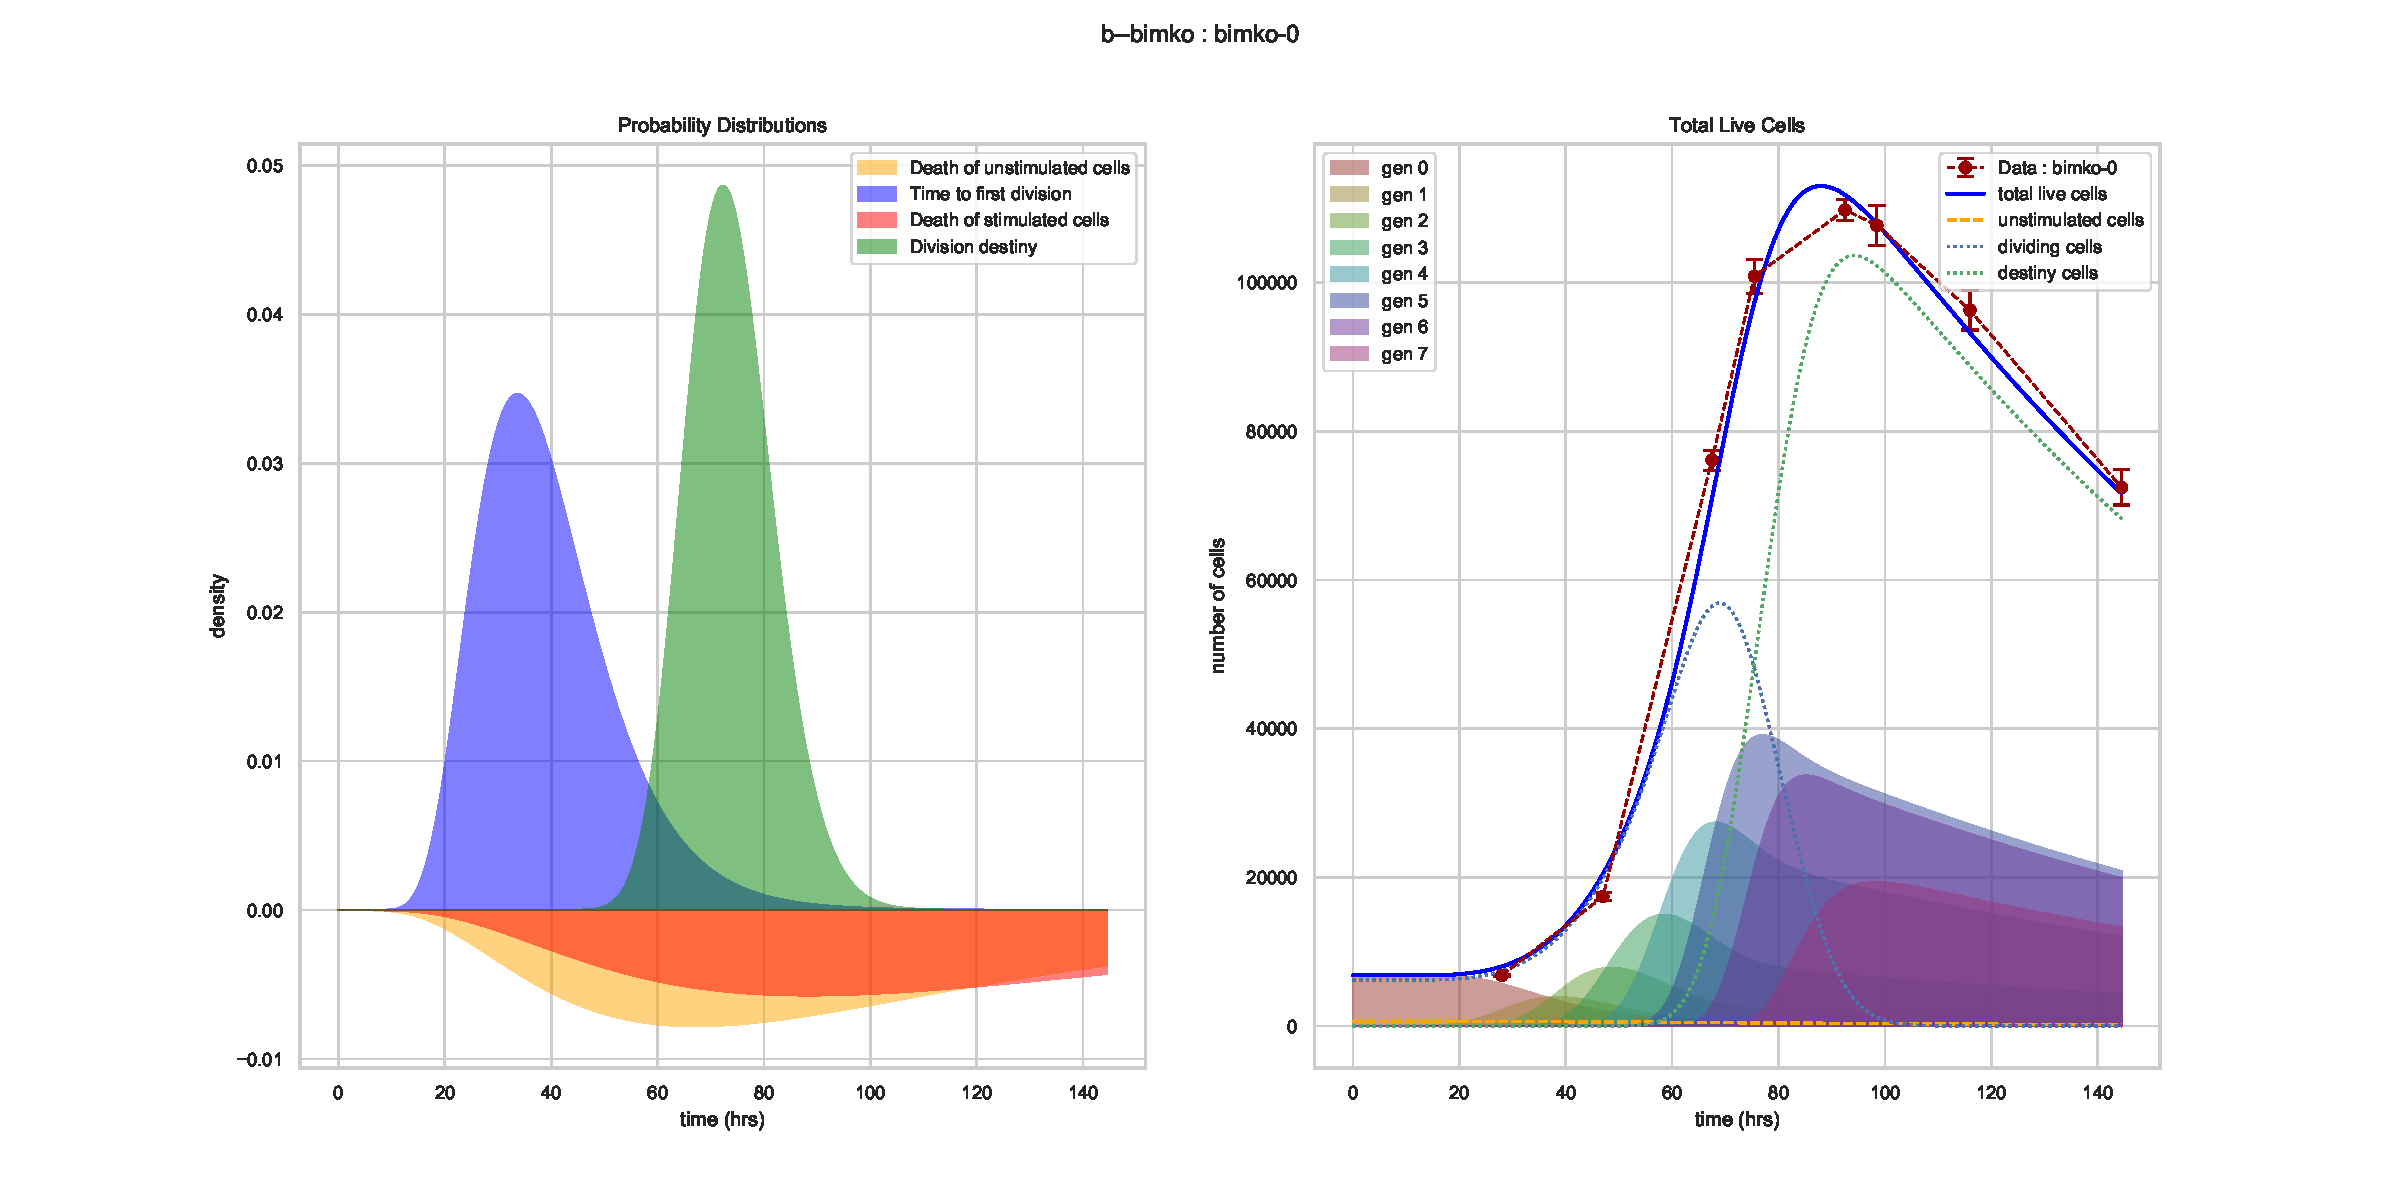
\includegraphics[scale=0.4]{./img/fig1_bimko-0.pdf}
                \caption{First export figure. Four probability distributions (\textit{LEFT}) and total live cell (\textit{RIGHT}, \textit{solid blue}) overlayed with live dividing \& destiny cells (\textit{dotted blue \& green} respectively), live cells at each generation (\textit{colored blocks}), and data point (\textit{dashed brown}). }
                \label{fig:fig1_export_plot}
            \end{subfigure}
            
            \begin{subfigure}{1\textwidth}
                \centering
                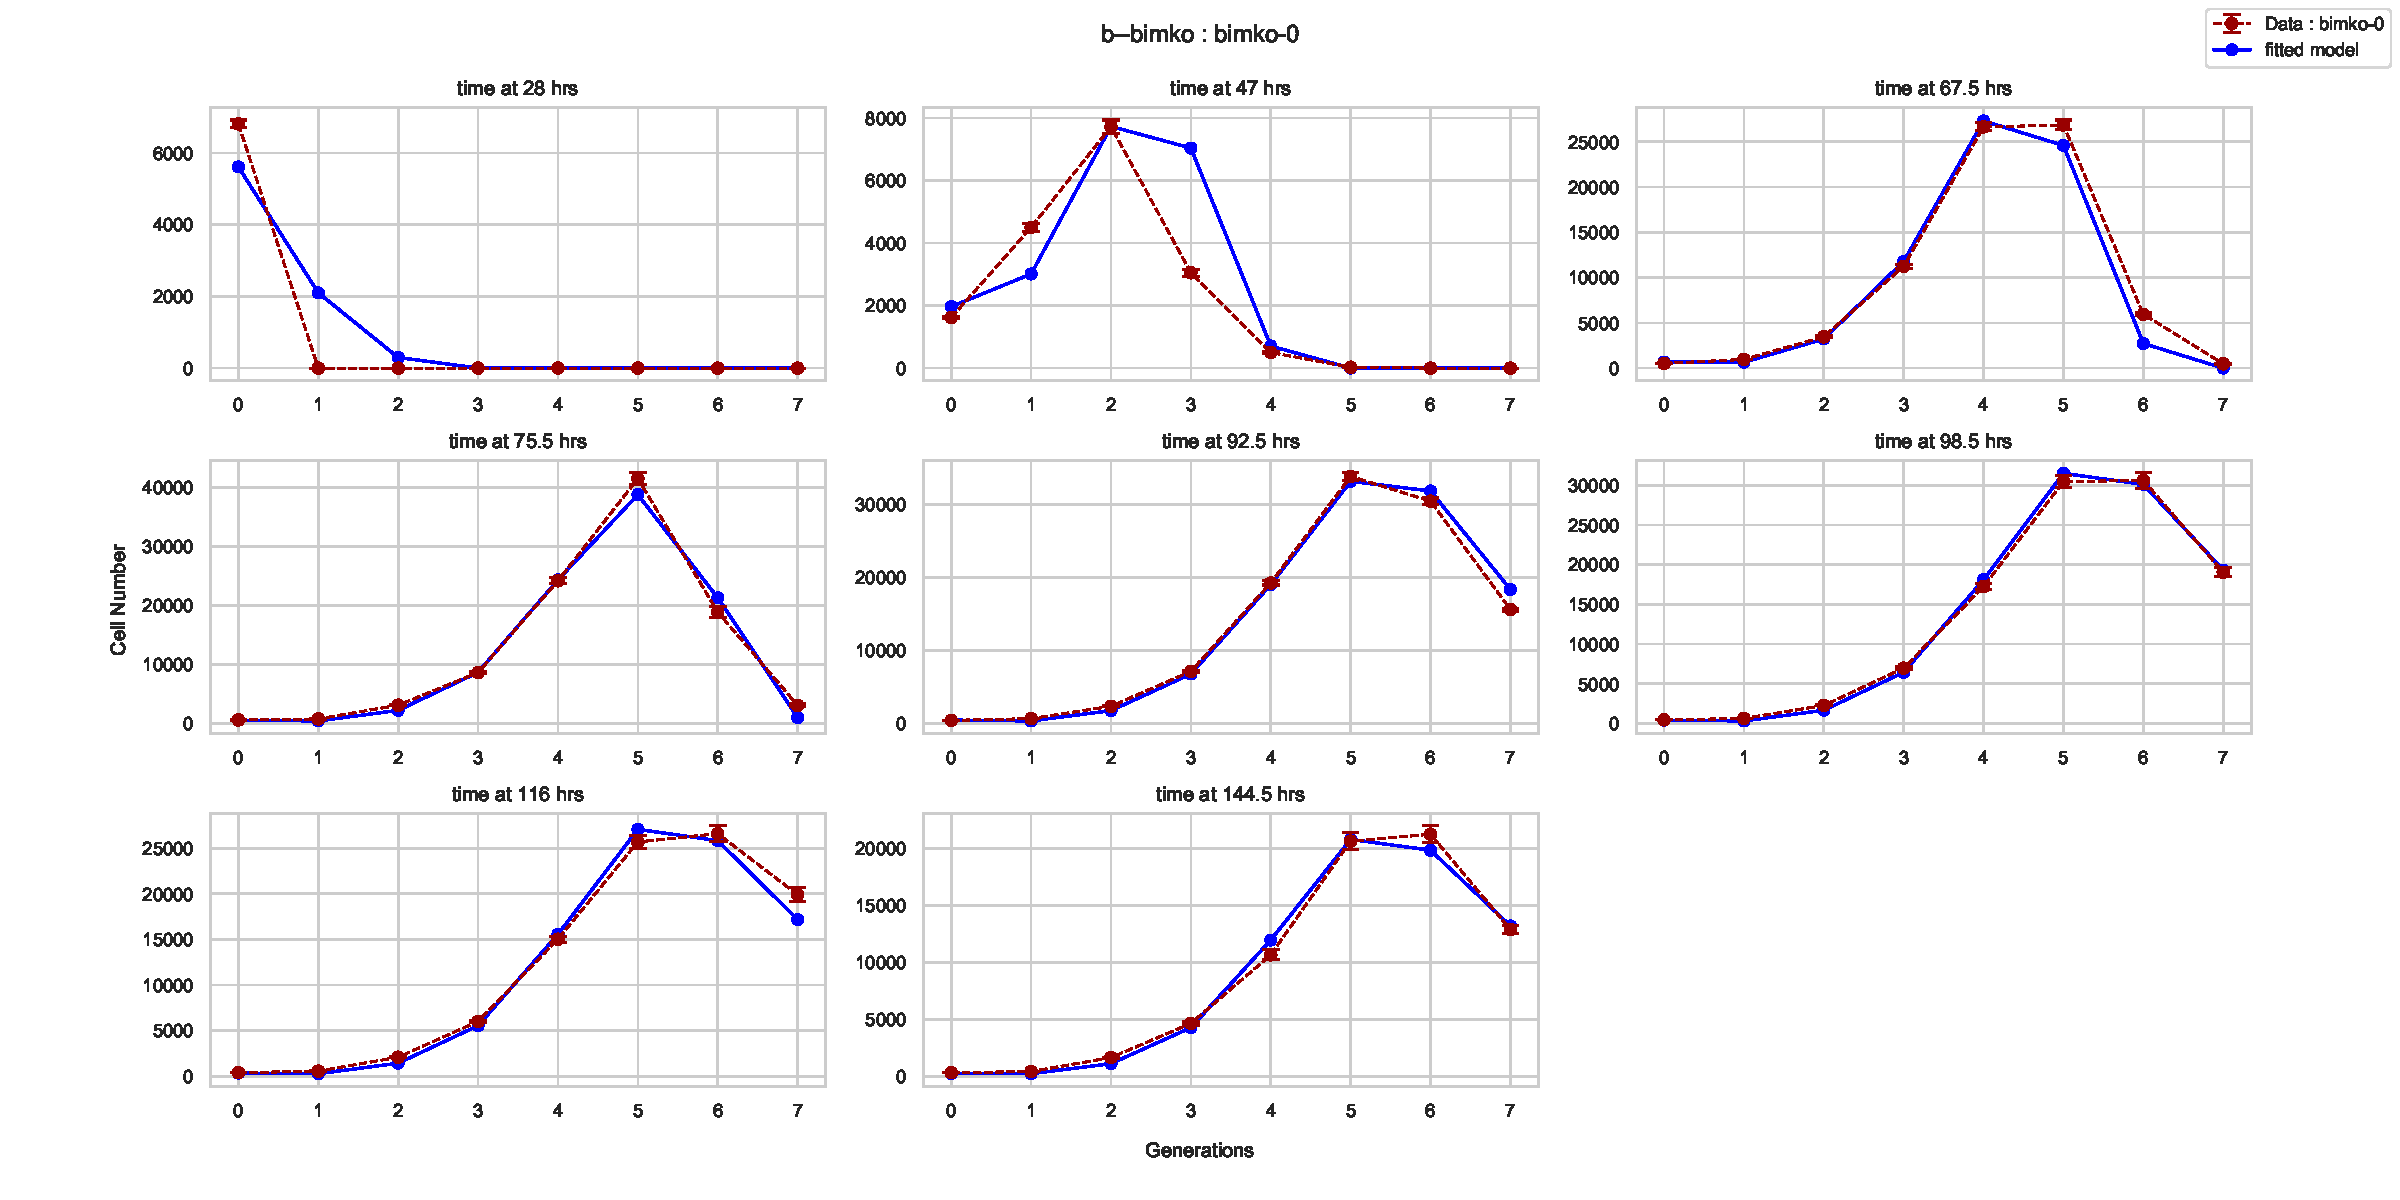
\includegraphics[scale=0.39]{./img/fig2_bimko-0.pdf}
                \caption{Second export figure. Overlayed plot of data (dashed brown) and total live cells (solid blue). Qualitative optimisation inspection can be done with this plot, unless you specify ``Fit to total cells''.}
                \label{fig:fig2_export_plot}
            \end{subfigure}
        \end{figure}

        \begin{figure}[h]\ContinuedFloat
            \begin{subfigure}{1\textwidth}
                \centering
                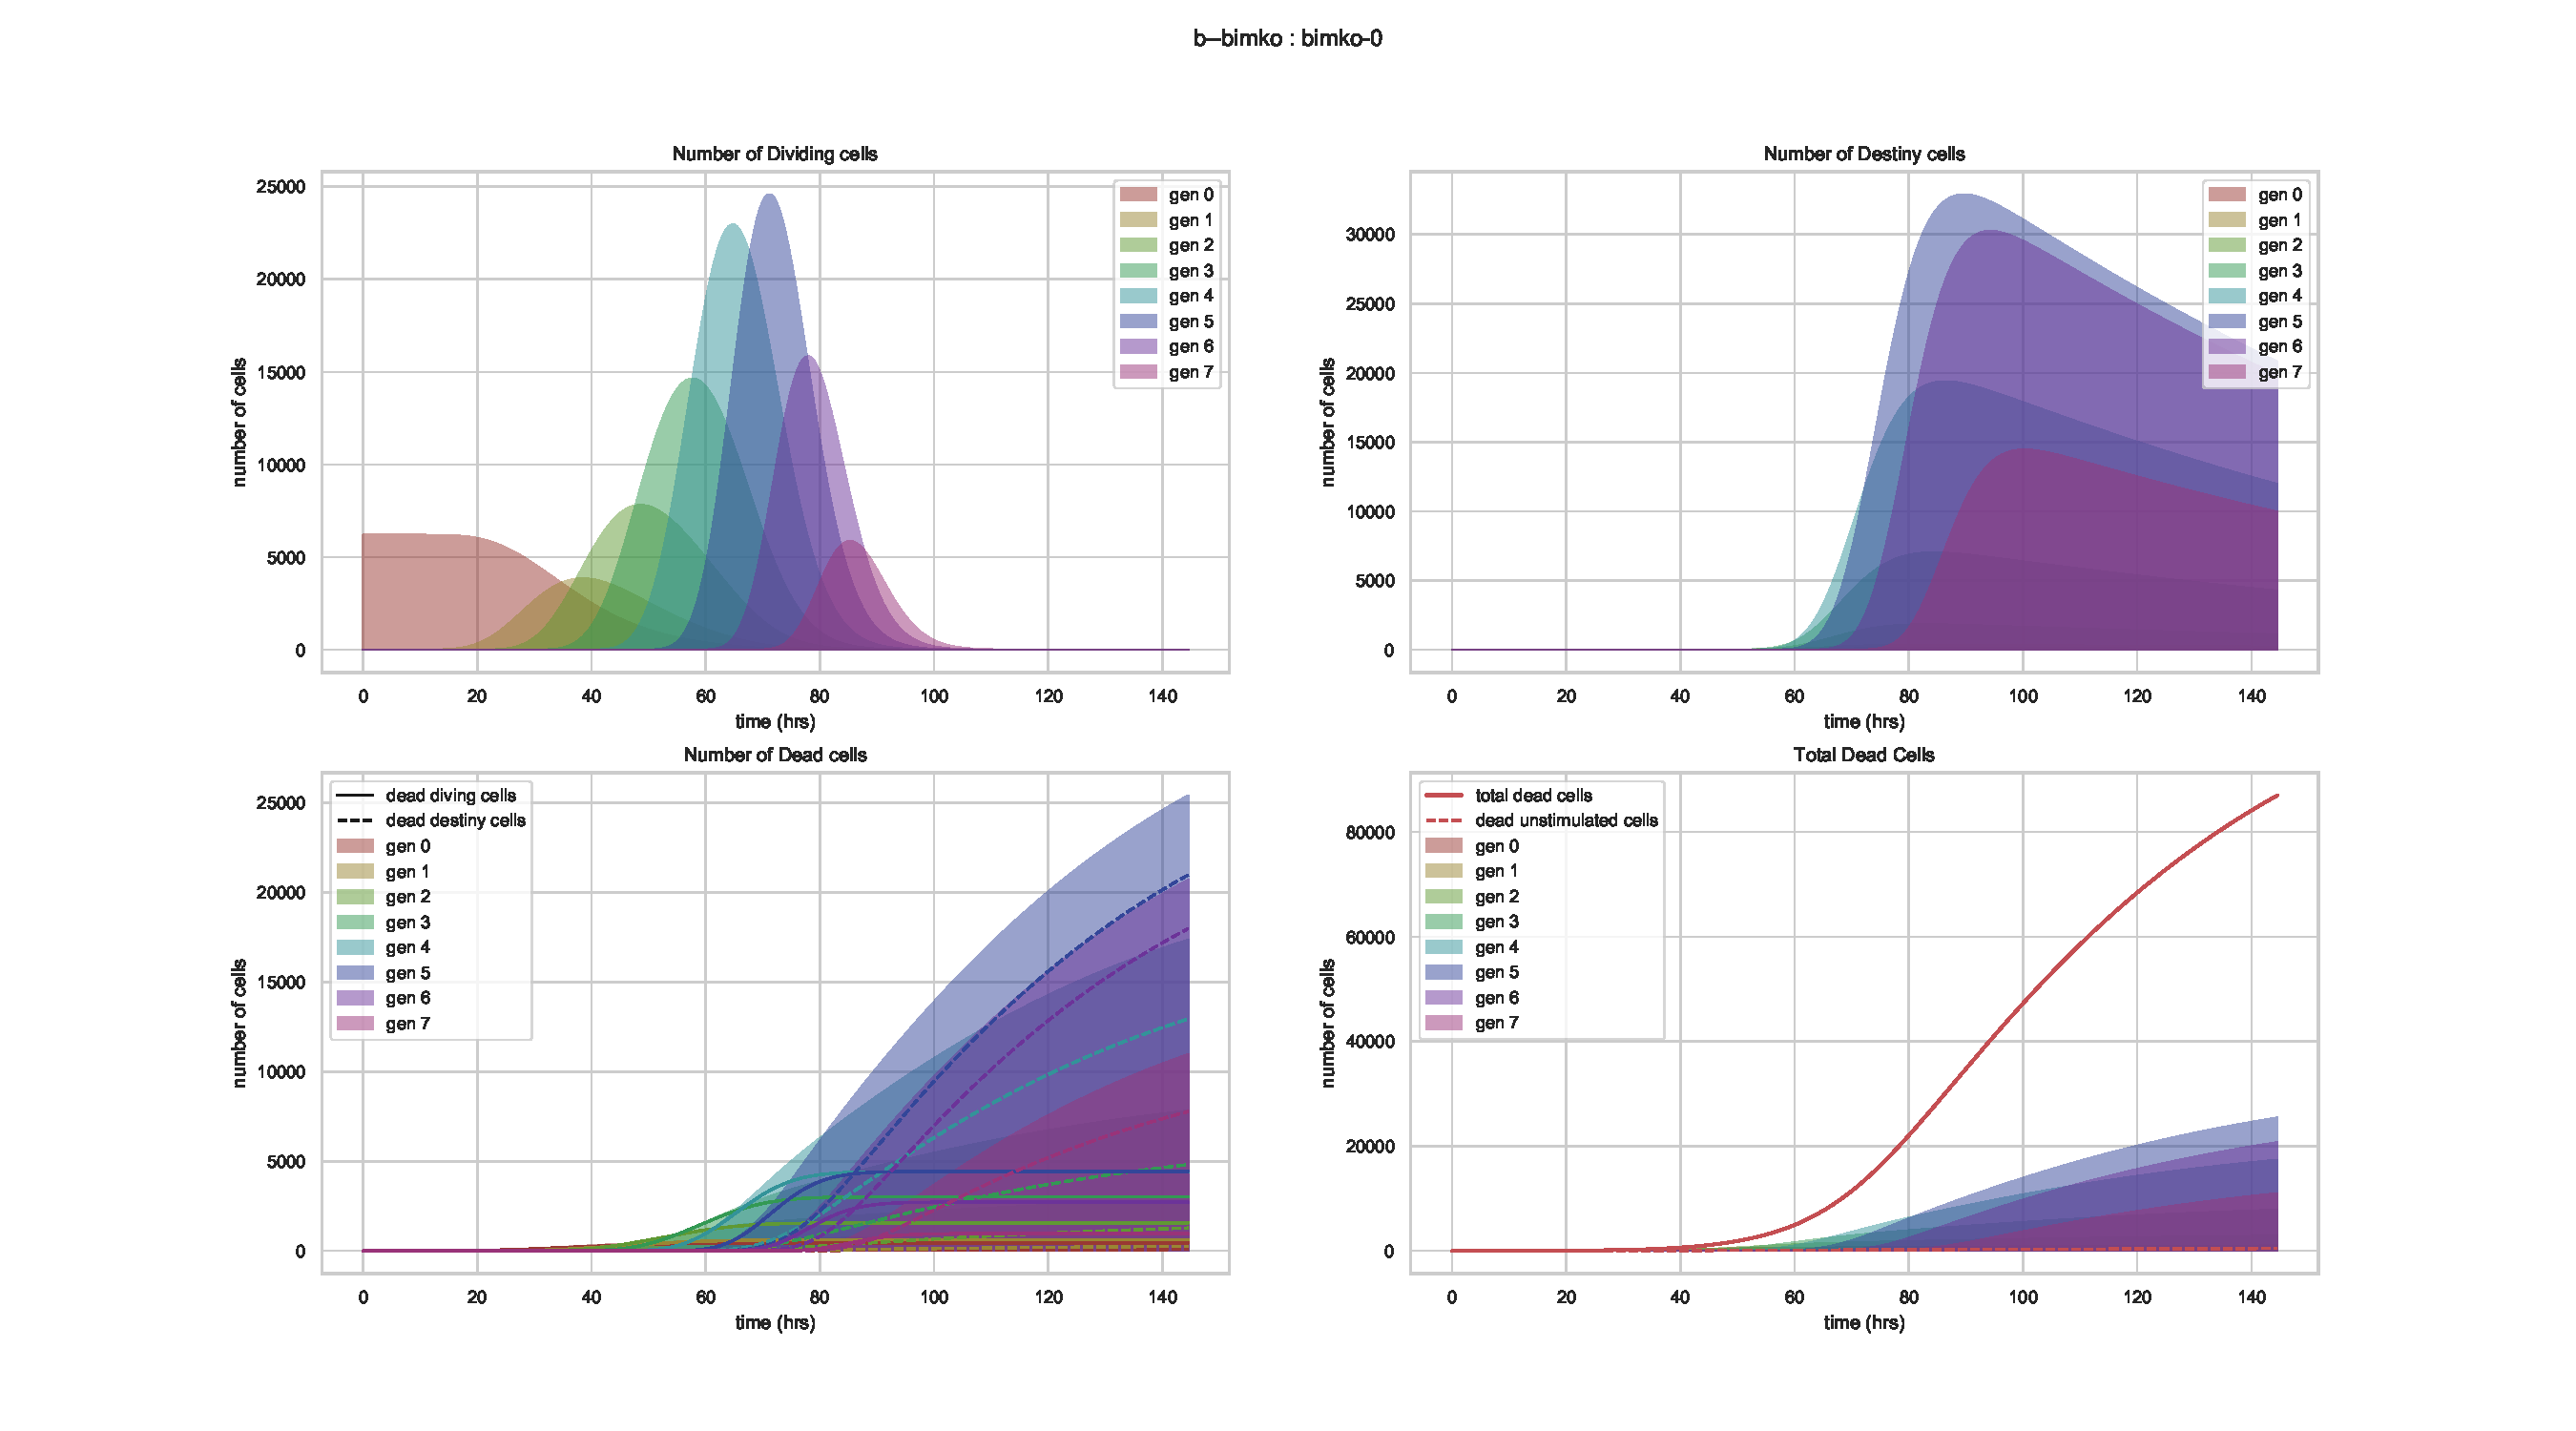
\includegraphics[scale=0.38]{./img/fig3_bimko-0.pdf}
                \caption{Third export figure. Hidden calculations are shown in here. Note that total live cells are composed of live ``dividing'' (\textit{TOP LEFT}) and destiny cells (\textit{TOP RIGHT}). Similarly, bottom two plots show cumulative dead ``dividing'' (\textit{solid colored}) and destiny (\textit{dashed colored}) cells (\textit{BOTTOM LEFT}) at any given time per generation.}
                \label{fig:fig3_export_plot}
            \end{subfigure}
            
            \begin{subfigure}{1\textwidth}
                \centering
                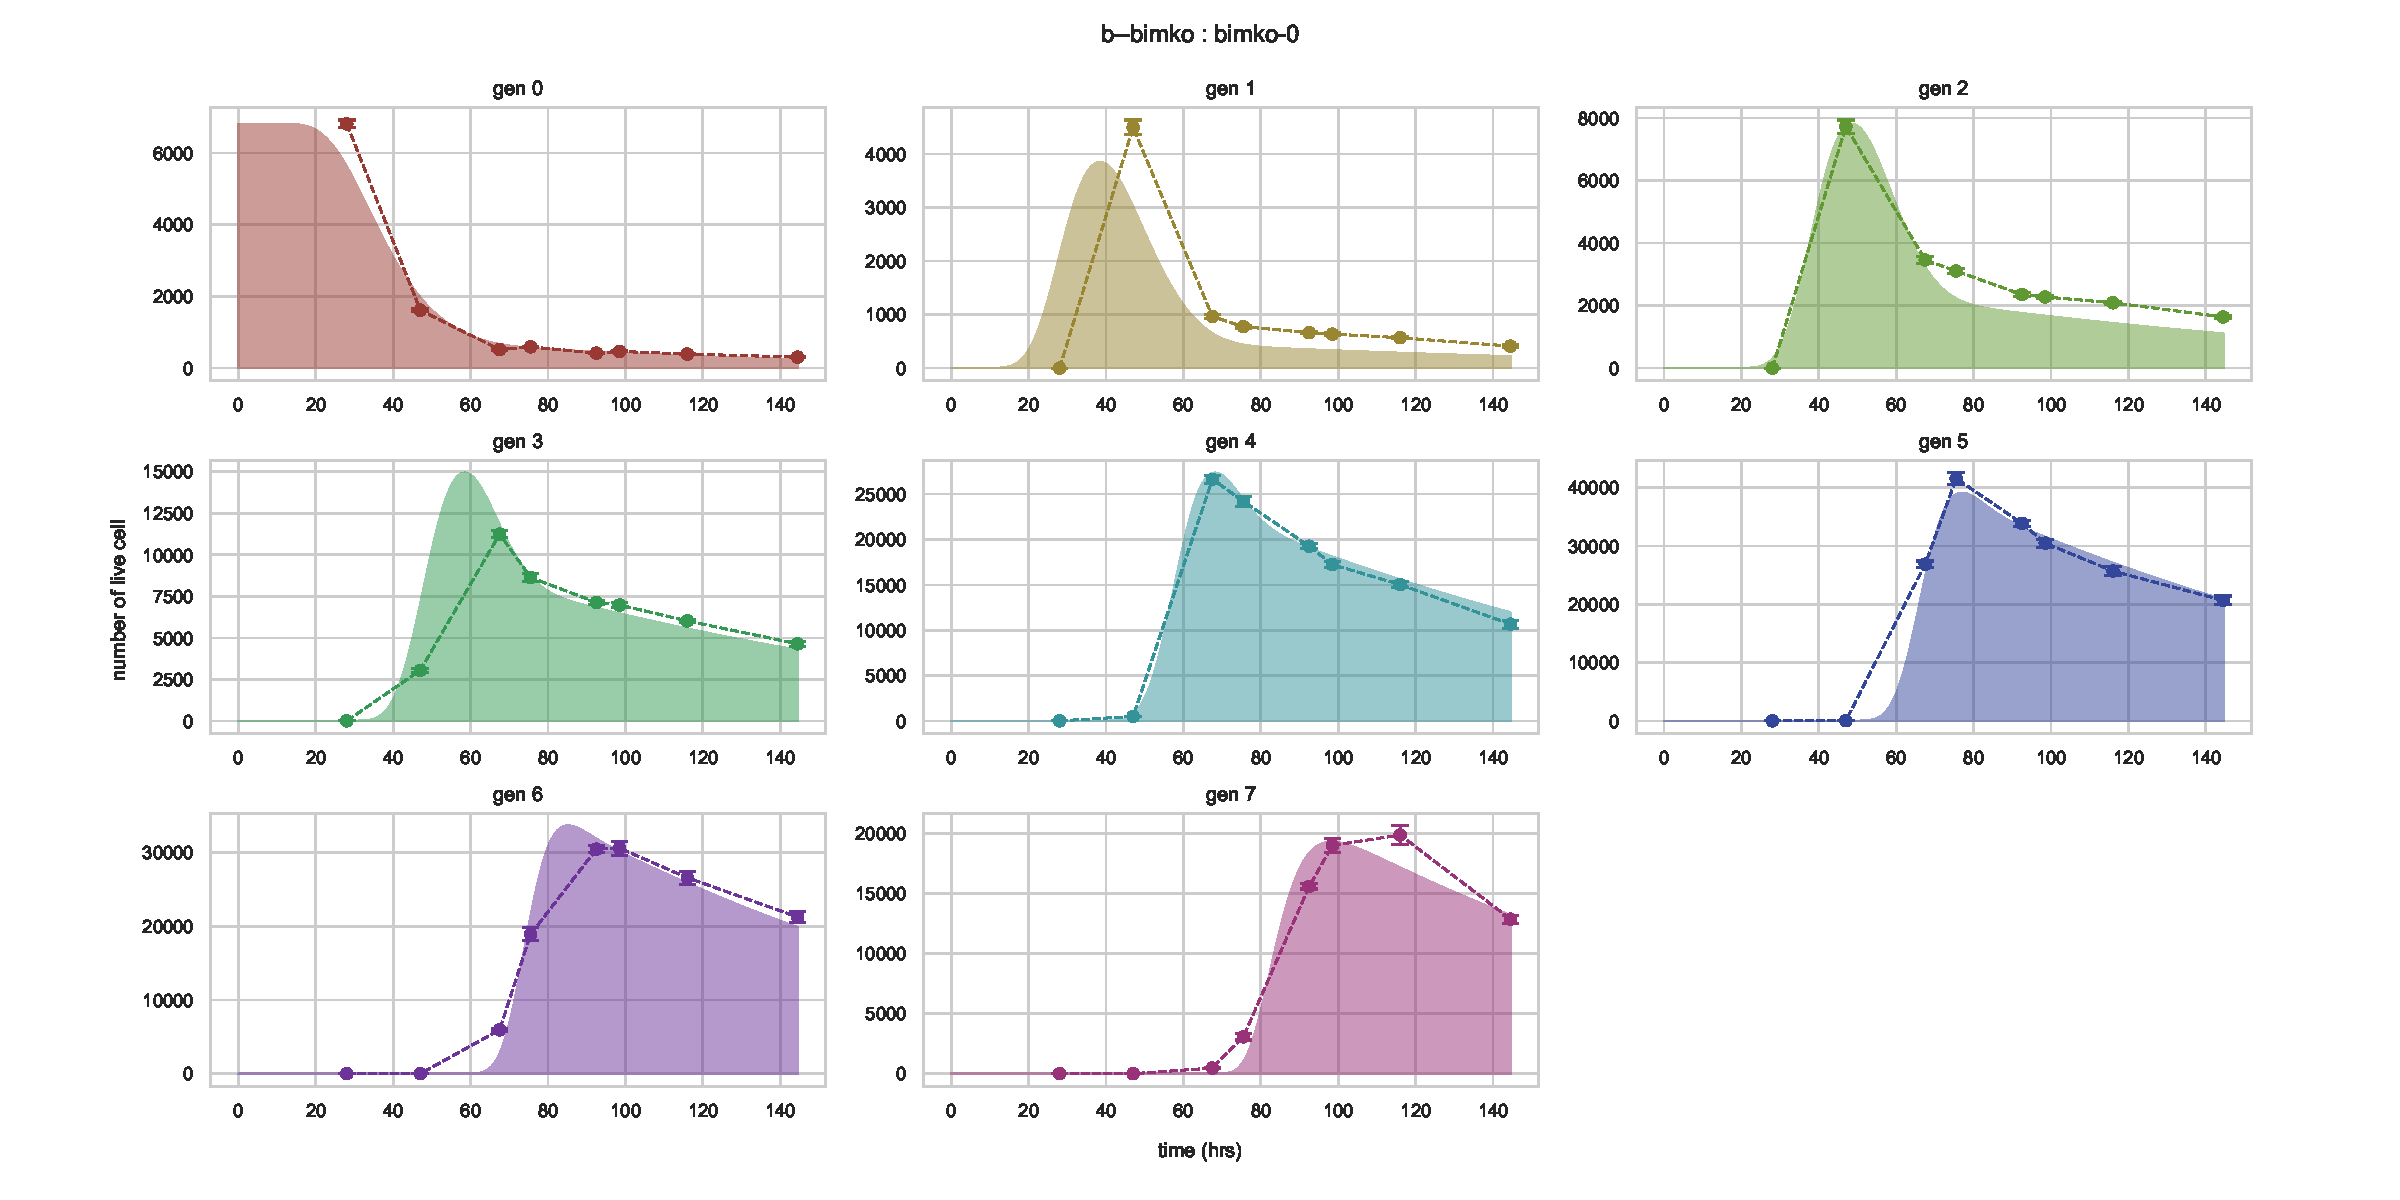
\includegraphics[scale=0.4]{./img/fig4-1_bimko-0.pdf}
                \caption{One of fourth export figures. The other one is exactly same as this except they are all overlayed in a single plot. Unlike Figure (\ref{fig:fig2_export_plot}), each panel represents total live cells per generation as a function of time. Data points are connected with \textit{dashed} line, and total live cells are \textit{colored blocks}.}
                \label{fig:fig41_export_plot}
            \end{subfigure}
            \caption{PDF files generated by \textbf{Export Plot} in the directory where input data file is. The program might get unreponsive while exporting due to heavy workload, so please wait for a success or error messages in the Console Log.}
            \label{fig:export_plot}
        \end{figure}

    \end{homeworkProblem}

    %---------------------------------------------------------------------------------
    %	SECTION 4 : About Cyton Model
    %---------------------------------------------------------------------------------
    \clearpage
    \begin{homeworkProblem}[Cyton Model]
        %-----------------------------------------------------------------------------
        %	SECTION 4.1 : Formalism
        %-----------------------------------------------------------------------------
        \subsection{Formalism}
        Let's assume that there exists functions such that we can compute live cell numbers, $N \in \mathbb{R}^+$, as function of time, $t \in [0, \infty)$, and generation, $i \in \mathbb{Z}^+$.
        \begin{equation}
            g_i (t) \rightarrow N,
        \end{equation}
        where $g$ is an arbitrary function to be speicified with various cellular machineries; typically encoded as a set of parameters. Indeed, one can raise a question that how a discrete quantity (e.g. number of cells) can be defined as a positive real number, but, for the purpose of creating a smooth continuous function, we will construct one that maps into real number space. This property might be important as we will discuss on some of optimisation protocols that require objective function to be differentiable everywhere. We also define $t=0$ to be beginning of the observation period. Based on this construction, it is worth noting that,
        \begin{equation}
            \sum_{i=0}^{i_{\mathrm{max}}} g_i(t) = G(t).
        \end{equation}
        Evidently $G(t)$ is \textit{total} number of live cells at time, $t$. $i_{\mathrm{max}}$ is a theoretical upper limit of division rounds. Ideally there are no apparent reason to put finite limit as some exotic cells (e.g. HeLa cells) undergo infinite number of cell division, however, in reality, we can typically track cell families up to seven or eight generation (experimental limitation of flow cytometry) and it has to be truncated for obvious numerical reason.

        We propose that there are four governing timers, which inherently consist of independent probability distributions, for each cellular activity. Overview of the population level calculation is shown in figure (\ref{fig:Cyton Model Summary}).

        In order to reduce parameters and improve fitting the subsequent division timer is not implemented as a random variable. Rather, it is a constant time equally applied for all sub-division rounds. A full stochastic model would incorporate variance in this parameter, however, we leave this as a future task.

        \begin{figure}[h]
            \centering
            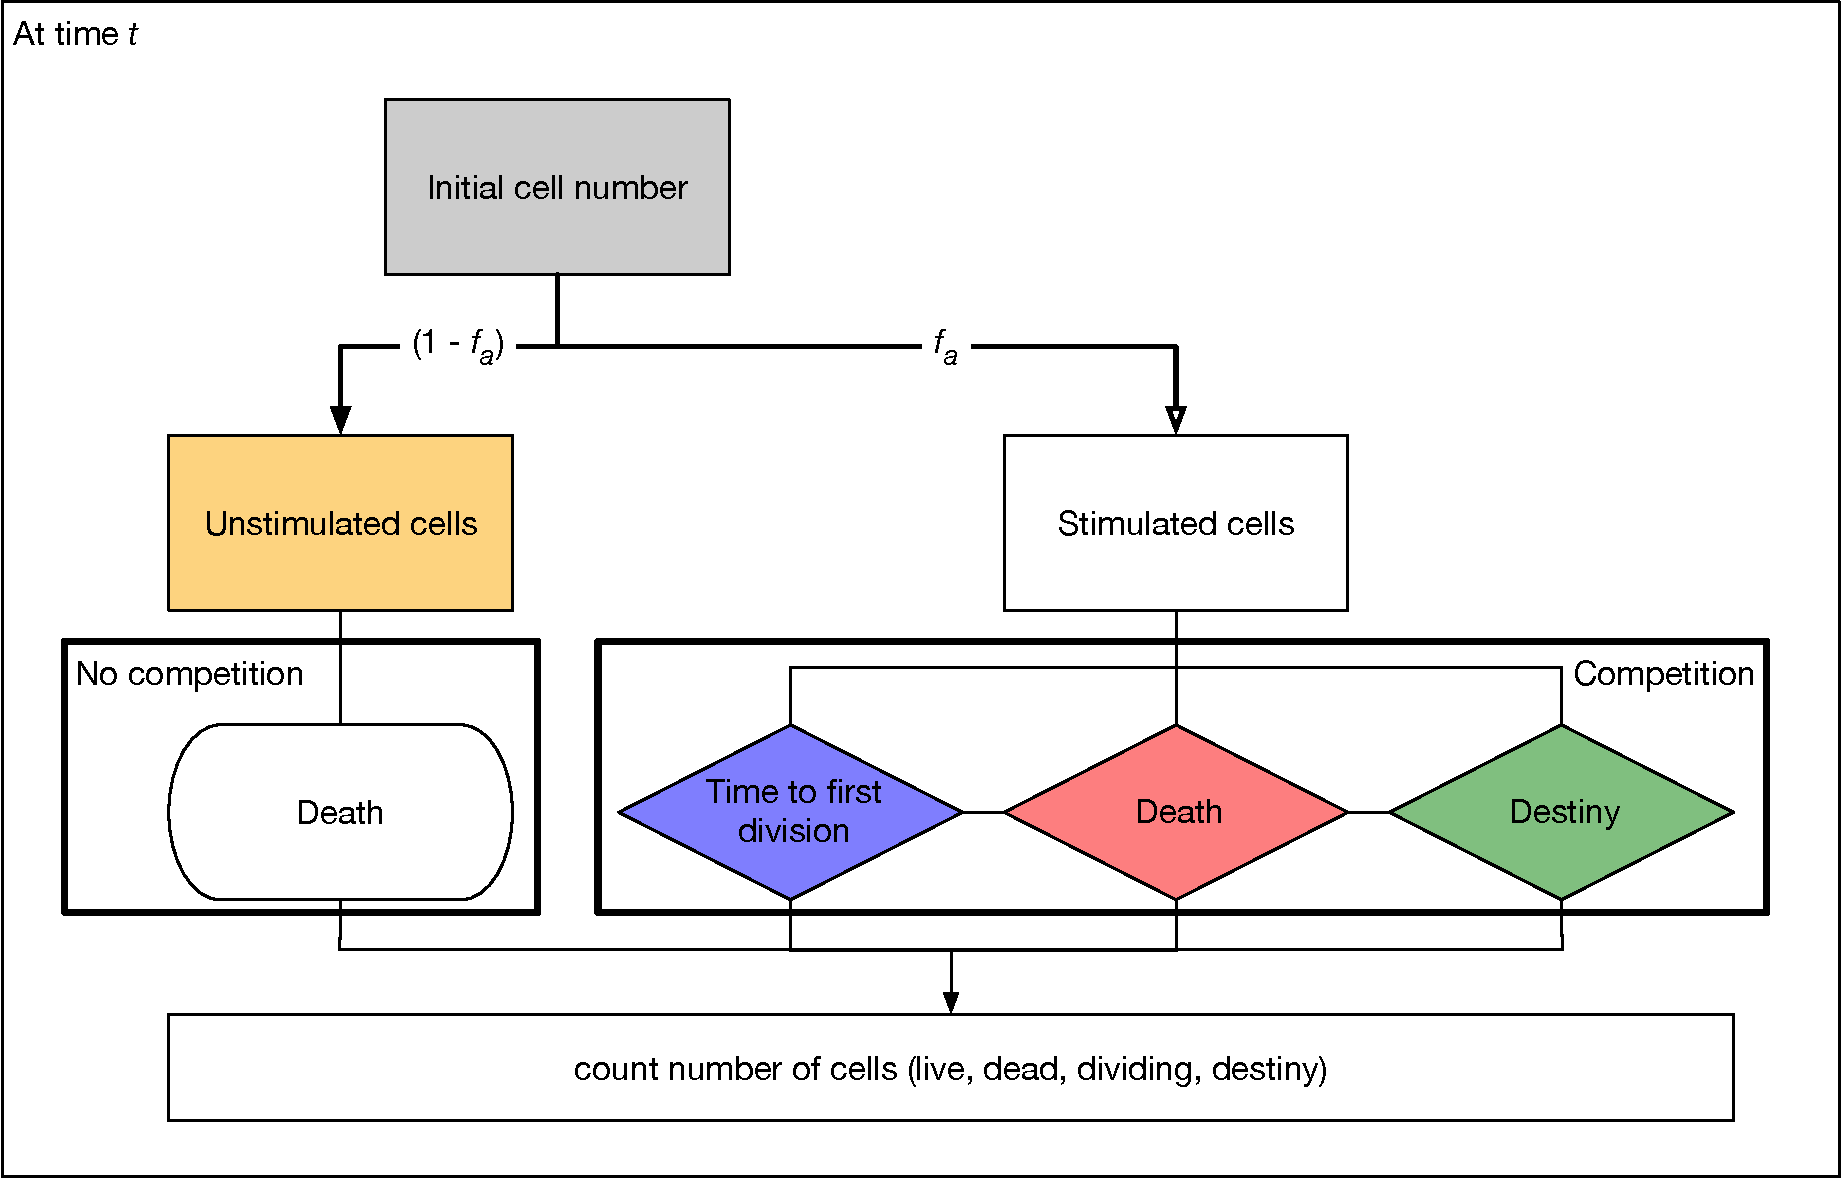
\includegraphics[scale=0.45]{./img/model_summary.pdf}
            \caption{Summary flow chart of cyton calculation. $f_a$ is an activation fraction (previously known as a progressor fraction, $pF$). Pool of cells are splitted into two groups, and they are subjected to either simple survival or competitive interaction.}
            \label{fig:Cyton Model Summary}
        \end{figure}
        
        The graphical representation of cyton 1.5 network is shown in the figure below,
        \begin{figure}[h]
            \centering
            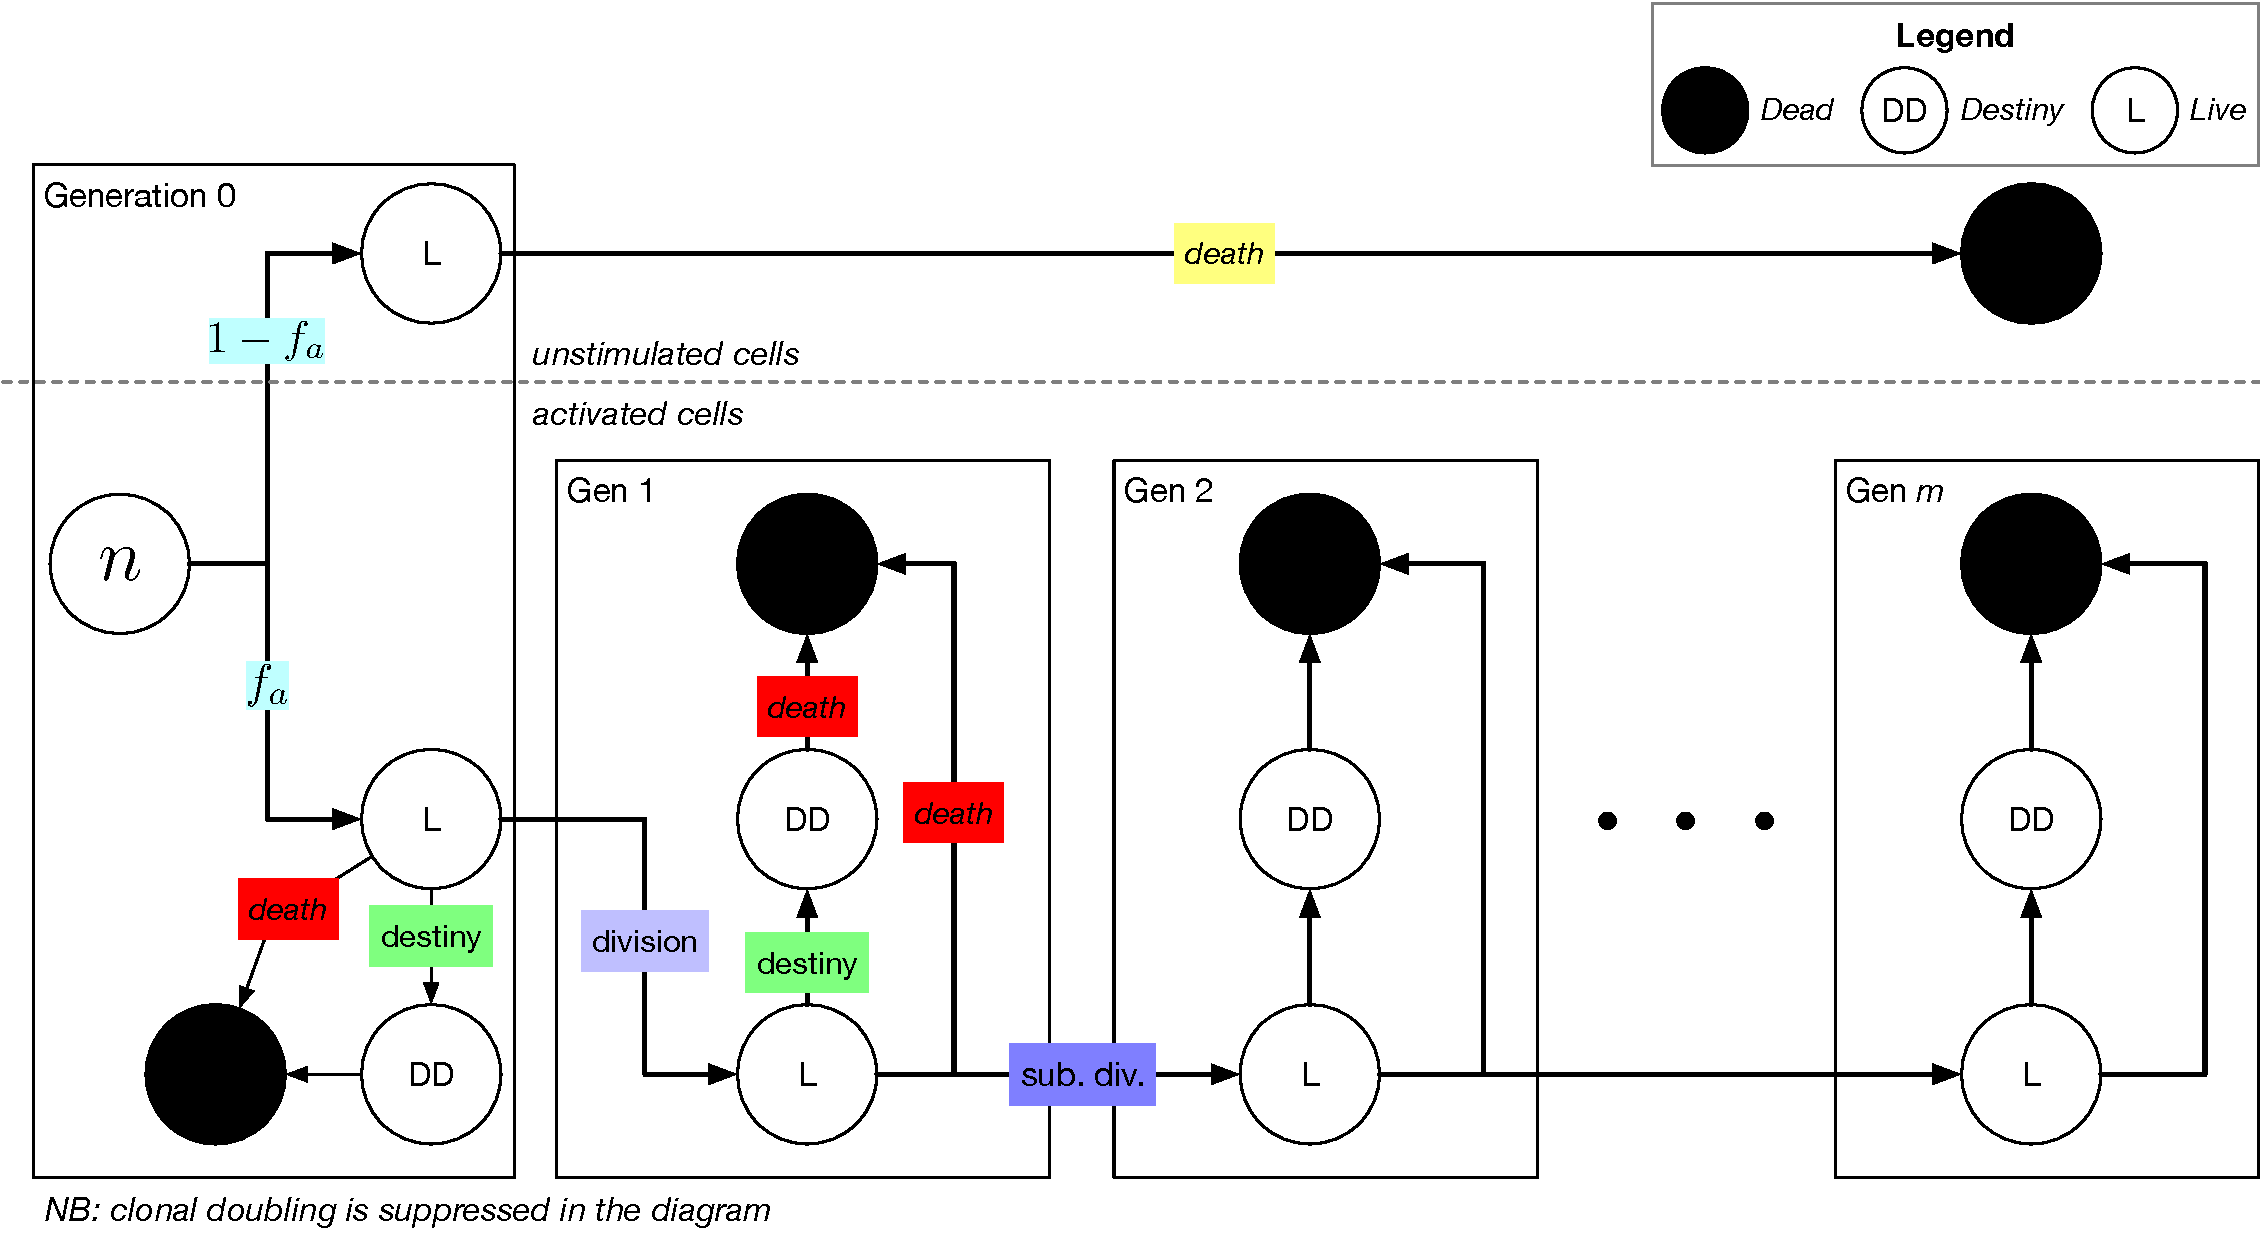
\includegraphics[scale=0.4]{./img/cyton_network.pdf}
            \caption{A decision making network of $n$ initial cell population. $f_a \in [0, 1]$ (\textit{cyan}) is an activation fraction that separates $n$ into unstimulated and activated groups. The probability distributions are assigned to each decisions (death time of unstimulated cells (\textit{yellow}), time to first division of activated cells (\textit{light blue}), death time of activated (\textit{red}), and time to division destiny (\textit{green})). Note that the subsequent division time (\textit{dark blue}) is not a random variable but a constant that equally applied for every generation $i\geq1$.}
            \label{fig:cyton_network}
        \end{figure}

        Following list shows assumptions and relevant parameters used in Cyton 1.5 model.\
        \begin{enumerate}
            \item \textbf{Initial cell number}, $n_0$. We define starting cell number to be a constant in this model, in general, that is,
            \begin{equation}
                G(0) = n_0.
            \end{equation}
            Employing biological intuition, we can expect that the model is neccessarily constrained to,
            \begin{equation}
                g_{i=0}(0) = n_0
            \end{equation}

            \item \textbf{Activation fraction}, $f_a \in [0, 1]$. A fraction of initial cells that undergoes division from generation 0 to 1; we define this fraction as \textit{stimulated}/\textit{activated} cells. These cells are subjected to the competition between next around of division, destiny, and death.
            \begin{equation}
                n_0^s = f_a \cdot n_0
            \end{equation}
            The other portion of cells (\textit{unstimulated}/\textit{inactivated}) are simply designed to follow death curve. By definition, we confine these quantities to exist only in generation 0.
            \begin{equation}
                n_0^u = (1 - f_a) \cdot n_0
            \end{equation}

            \item \textbf{Death timer for unstimulated}, $D = LogN(\mu_D, \sigma_D) \ \mathrm{or} \ N(\mu_D, \sigma_D)$. A non-competitive probability distribution, which is responsible for death of unstimulated cells.
            
            \item \textbf{Time to first division timer}, $\phi = LogN(\mu_{\phi}, \sigma_{\phi})\ \mathrm{or} \ N(\mu_{\phi}, \sigma_{\phi})$. A competitive probability distribution for stimulated/activated cells in generation 0. They are allowed to enter the first round of division accordingly.
            
            \item \textbf{Death timer for stimulated}, $\psi = LogN(\mu_{\psi}, \sigma_{\psi})\ \mathrm{or} \ N(\mu_{\psi}, \sigma_{\psi})$. A second competitive probability distribution for stimulated/activated cells in \textit{all} generations. Therefore, we assume that the death rates are equally shared for all clonal cells. This is different and independent death distribution to that of unstimulated one.
            
            \item \textbf{Destiny timer}, $\xi = LogN(\mu_{\xi}, \sigma_{\xi})\ \mathrm{or} \ N(\mu_{\xi}, \sigma_{\xi})$. Last competitive probability distribution for stimulated/activated cells in \textit{all} generations. When the timer expires before other competing timers, cells enter quiescence state and are no longer part of division path way, but still under influence of death timer.
            
            \item \textbf{Subsequent divsision timer}. $b$. It is the time that cells take to traverse each subsequent division. We assume that time in between each division is equally separated, and is unaffected by the time to first division. As a consequence the time to generation $i$ will be identical to,
            \begin{equation}
                \mu_{\phi} + i \cdot b \quad \forall \quad i=[1, 2, \dots, i_{\mathrm{max}}]
            \end{equation}
        \end{enumerate}
        In summary, we have total of ten parameters in the model,
        \begin{equation}
            \mathbf{\hat{p}} = \{f_a, b, (\mu_D, \sigma_D), (\mu_{\phi}, \sigma_{\phi}), (\mu_{\psi}, \sigma_{\psi}), (\mu_{\xi}, \sigma_{\xi})\}
        \end{equation}
        such that our objective function is parameterised as,
        \begin{equation}
            g_i(t) = g_i(t;\mathbf{\hat{p}})
        \end{equation}

        %----------------------------------------------------------------------------------------
        %	SECTION 4.2 : Construction of the Model
        %----------------------------------------------------------------------------------------
        \subsection{Construction of the Model}
        In this section, we discuss what constitutes the model based on the assumptions and parameters shown previously.

        Given unstimulated probability distribution, $D(t;\mu_D, \sigma_D)$, we can calculate number of live cells,
        \begin{equation} \label{eq:unstim_gen0}
            N_{i=0}^u (t) = n_0^u \left(1 - \int_0^t D(t')dt'\right)
        \end{equation}
        Essentially it is a monotonically decreasing survival function (c.f. Figure(\ref{fig:example_unstimulated_cell_survival})).
        \begin{figure}[h]
            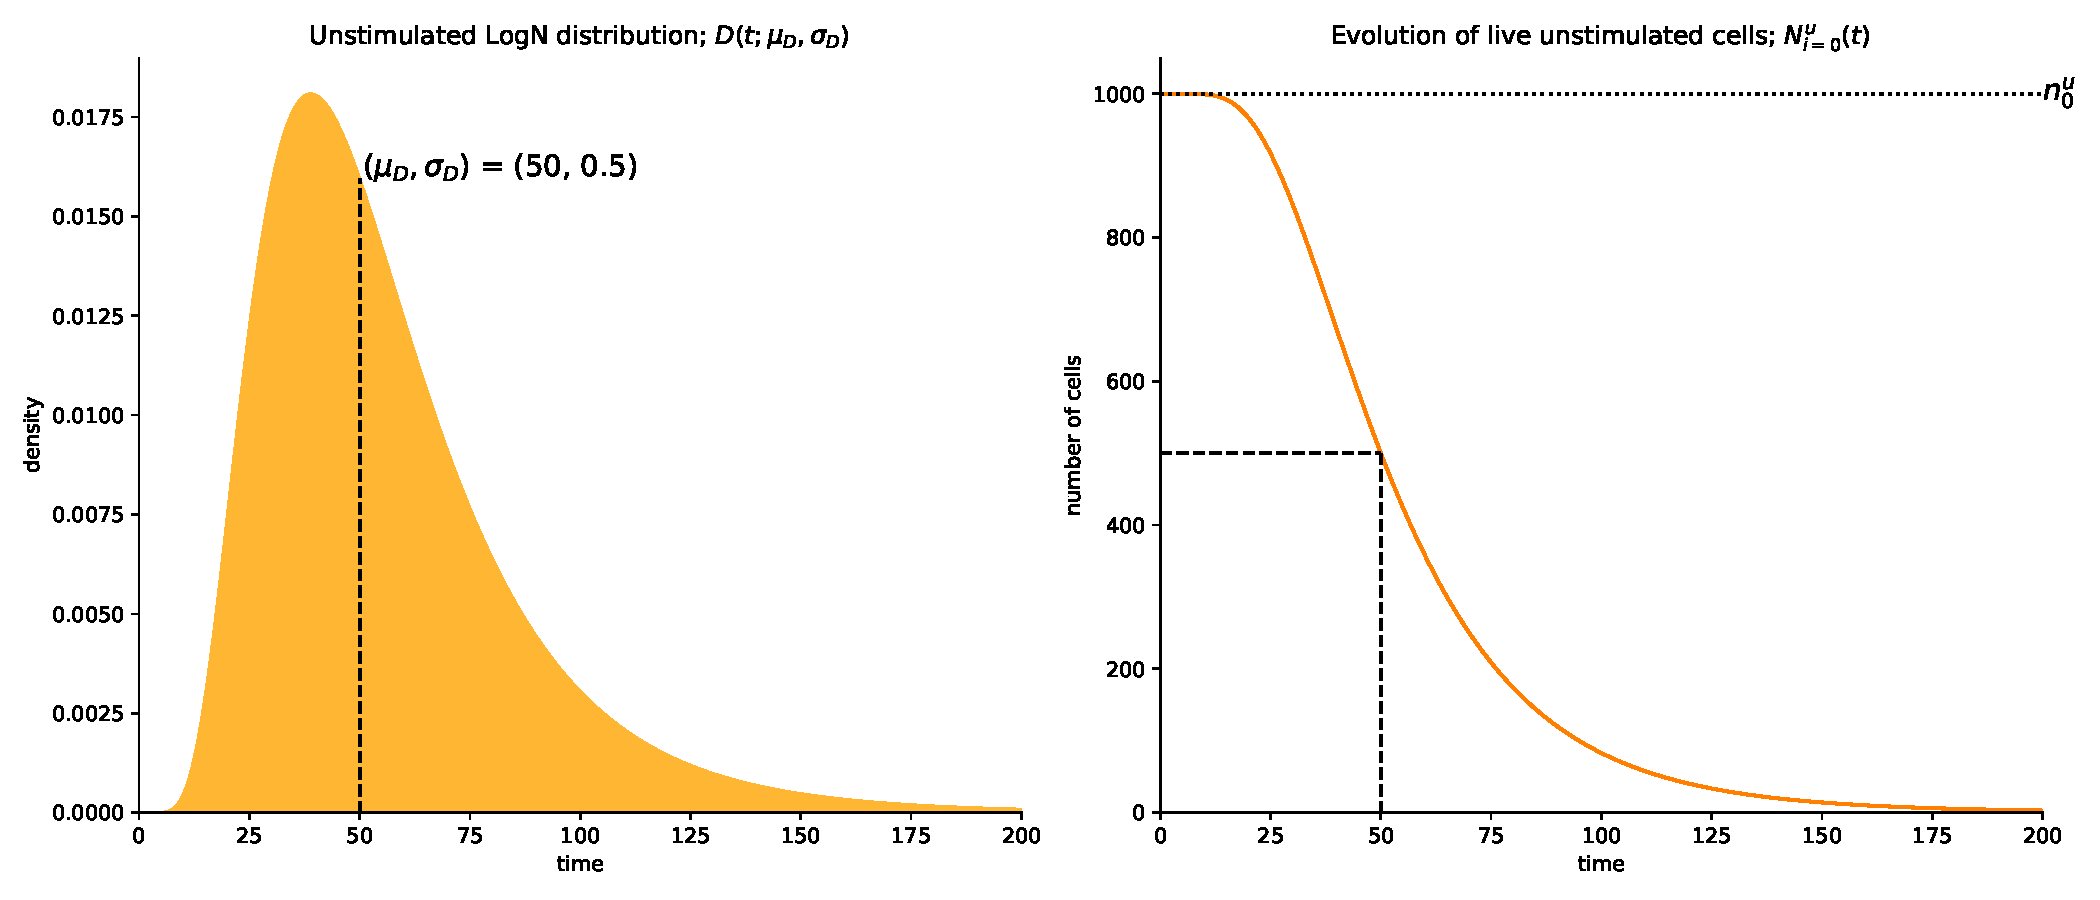
\includegraphics[scale=0.43]{./img/ex_unstim.pdf}
            \centering
            \caption{An example dynamic of unstimulated cells following a Log-Normal death distribution.}
            \label{fig:example_unstimulated_cell_survival}
        \end{figure}

        Similarly, we can compute two states of live stimulated cells; dividng and destiny cells. For dividing cells, we take away cells that would have died, entered first division, and reached destiny from the initial stimulated cells ($n_0^s$). Whereas, destiny cells are computed cumulatively such that once cells reach destiny they do not enter further division rounds and await for their death.
        \begin{align}
            N_{i=0}^{div} (t) & = Q(t) \left(1 - \int_0^t \xi(t')dt'  \right) \left(1 - \int_0^t \phi(t')dt' \right), \label{eq:stim_gen0-div} \\
            N_{i=0}^{dd} (t) & = Q(t) \int_0^t \xi(t') \left(1 - \int_0^{t'} \phi(\tau) d\tau \right) dt' \label{eq:stim_gen0-dd}
        \end{align}
        where $Q(t) = n_0^s \left(1 - \int_0^t \psi(t')dt' \right)$. Figure(\ref{fig:stim-gen0}) illustrates three possible configurations for $\phi(t)$ and $\xi(t)$ assuming that $Q(t)=n_0^s$ is constant, i.e. no death. Loss of cells indicates that they proceed to first division. Introducing death distribution back into the equation would show decrease in cell number for both dividing and destiny curves simultaneously.
        \begin{figure}[h]
            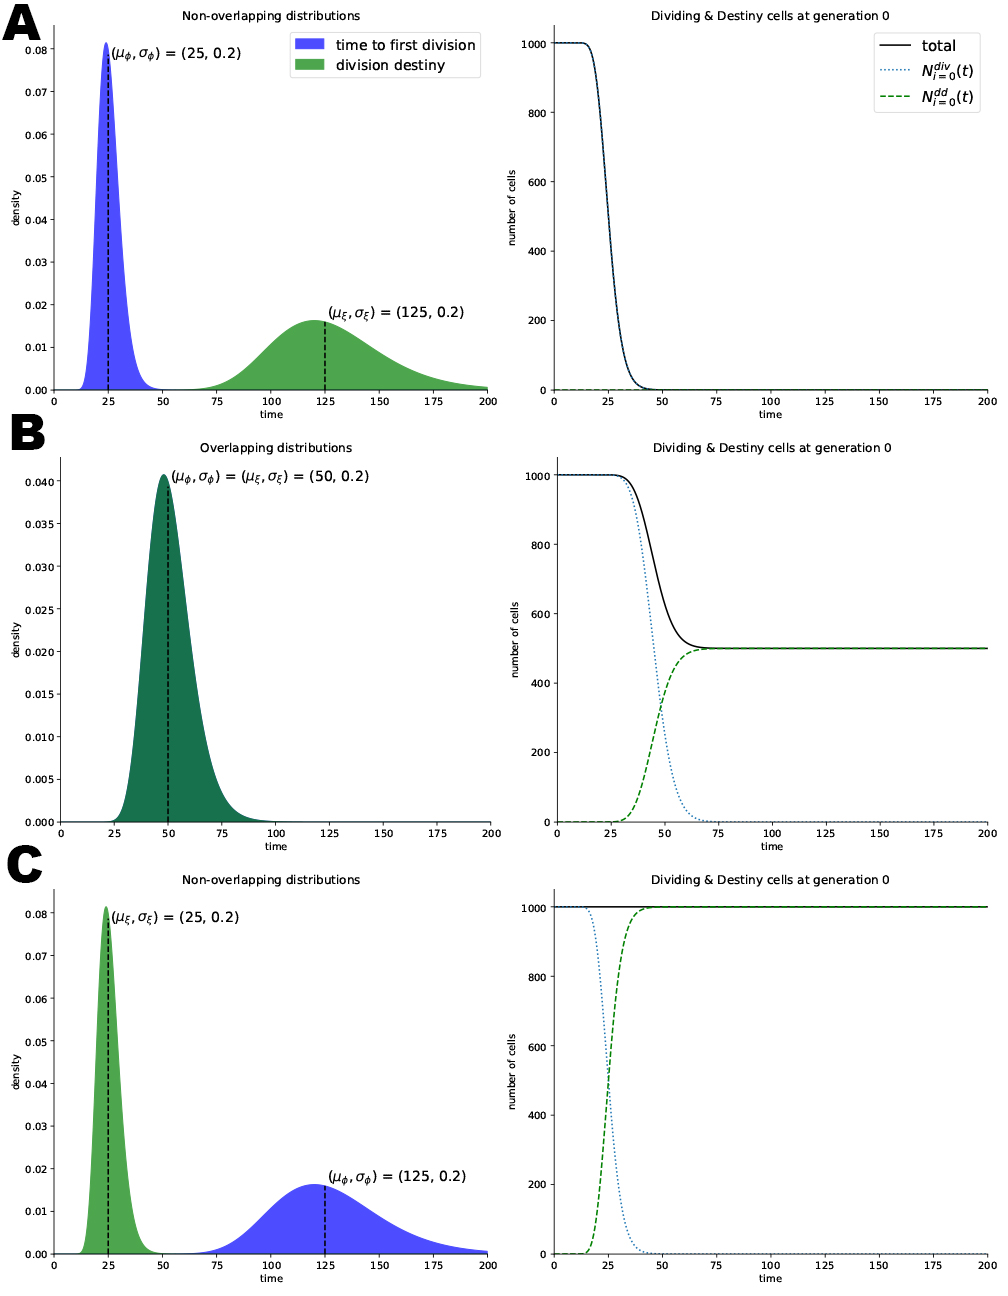
\includegraphics[scale=0.42]{./img/stim-gen0-combined.jpg}
            \centering
            \caption{Effects of competition between division and destiny in absence of death ($t_{\mathrm{death}} \gg t_{\mathrm{tfd}}, t_{\mathrm{dd}}$). Each row contains distribution configuration (\textit{LEFT}) and live cells at generation 0 (\textit{RIGHT}). Dotted blue line is dividing cells ($N_{i=0}^{div}$), dashed green line is destiny cells ($N_{i=0}^{dd}$), and solid black line is total live cells. (A) Cells are highly likely to enter first round of division before reaching destiny. This effect is shown as decrease in number of dividing cells as well as total. (B) Two coinciding distributions. If we configured them to be identically equal, we can expect half of the cells will reach destiny while the other half enter the division. (C) Cells are highly likely to to reach destiny. This effectively censors cells from entering first division, and converting cell state from dividing to destiny, therefore there are no change of total live cells.}
            \label{fig:stim-gen0}
        \end{figure}

        Summing all equations (\ref{eq:unstim_gen0}), (\ref{eq:stim_gen0-div}), (\ref{eq:stim_gen0-dd}), we obtain total live number of cells at generation 0,
        \begin{equation} \label{eq:g_gen0}
            g_{i=0}(t;\mathbf{\hat{p}}) = N_{i=0}^u(t) + N_{i=0}^{div}(t) + N_{i=0}^{dd}(t)
        \end{equation}
        For generations, $i>0$, the number of dividing or destiny cells are given by,
        \begin{align}
            N_{i>0}^{div}(t) & = 
            \begin{cases}
                2^i \cdot Q(t) \left(1 - \int_0^t \xi(t')dt'\right) \int_0^{t-(i-1)b} \phi(t')dt' & \mathrm{if} \quad (i-1)b < t \leq i \cdot b \\
                2^i \cdot Q(t) \left(1 - \int_0^t \xi(t')dt' \right) \int_{i\cdot b}^t \phi(t')dt' & \mathrm{if} \quad  t > i \cdot b
            \end{cases} \\
            N_{i>0}^{dd}(t) & =
            \begin{cases}
                2^i \cdot Q(t) \int_0^t \xi(t') \left(\int_0^{t'-(i-1)b}\phi(\tau)d\tau\right)dt' & \mathrm{if} \quad (i-1)b < t \leq i \cdot b \\
                2^i \cdot Q(t) \int_0^t \xi(t') \left(\int_{i\cdot b}^{t'}\phi(\tau)d\tau\right)dt' & \mathrm{if} \quad t > i\cdot b
            \end{cases}
        \end{align}
        They almost resemble the equations (\ref{eq:stim_gen0-div}) and (\ref{eq:stim_gen0-dd}) except we imposed time constraints on each expression to define periods at which cells are allowed to traverse subseuqent division. It essentially regulates the time and proportion of cells entering from division $i$ to $i+1$. Calculating dividing cells is carried by obtaining the proportion of cells that would have entered generation $i$ with clonal factor $2^i$, and subtract number of cells that would have died and reached destiny. Similarly, destiny cells are calculated cumulatively from proportion of cells that entered $i^{th}$ generation. Notably, provided that full description of cellular machineries, our formulation suggests that each operation at time, $t$, is non-recursive unlike previous cyton model. It requires no prior knowledge to compute exact number of cells regardless of their states.

        Figure(\ref{fig:stim-gen-pp}) illustrates the model progression of cell division with (A) 2-way competition configuration between $\phi(t)$, $\xi(t)$, and $b$. As a consequence of absence of death, it is obvious that the cell numbers reach plateau as destiny stops them from diverging to infinity. (B) 3-way competition configuration where we adopted same parameter values for $\phi(t)$, $\xi(t)$, and $b$ subjected in Figure(\ref{fig:stim-gen-pp}A), except the death is now included. We truncated the model at $i_{max} = 7$ for visual purposes.

        Adding the equation of two states yields total number of cells at generation $i>0$,
        \begin{equation}\label{eq:g_gen>0}
            g_{i>0} (t) = N_{i>0}^{div}(t) + N_{i>0}^{dd}(t).
        \end{equation}
        Therefore, the objective function is defined by combining equation (\ref{eq:g_gen0}) and (\ref{eq:g_gen>0}),
        \begin{equation} \label{eq:all}
            g_i(t;\mathbf{\hat{p}}) =
            \begin{cases}
                N^{div}(t) + N^{dd}(t) + N^u(t) & \mathrm{if} \ i=0 \\
                N^{div}(t) + N^{dd}(t) & \mathrm{if} \ i > 0
            \end{cases}
        \end{equation}

        \begin{figure}[h]
            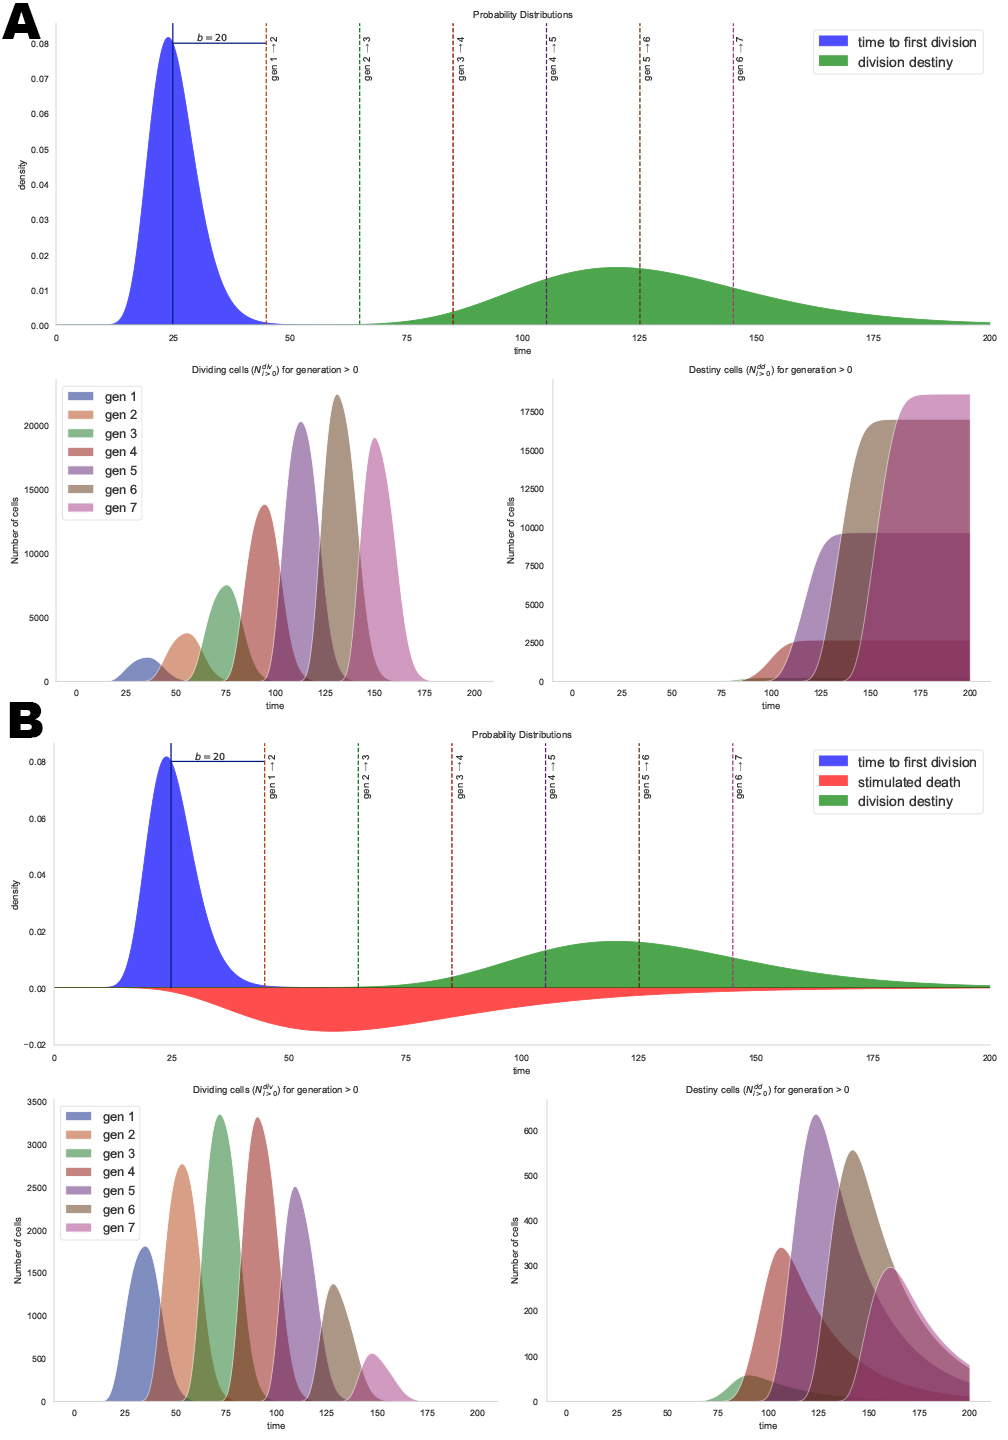
\includegraphics[scale=0.41]{./img/stim-combined.jpg}
            \centering
            \caption{Competition of time to first division, destiny, and death for stimulated cells. (A) Cells are allowed to remain in resting state for indeinite period. We can observe that each peak in dividing cell plot is doubled until they reached destiny. (B) Number of cells that are entering subsequent division is reduced due to cell death while in dividing state. The destiny cells are also simultaneously subjected to the death, exhibiting lognormal tail at the end.}
            \label{fig:stim-gen-pp}
        \end{figure}
        
        %----------------------------------------------------------------------------------------
        %	SECTION 4.3 : Optimisation Strategy
        %----------------------------------------------------------------------------------------
        \subsection{Optimisation Strategy}
            %----------------------------------------------------------------------------------------
            %	SECTION 4.3.1 : Least-squares Problem
            %----------------------------------------------------------------------------------------
            \subsubsection{Least-squares Problem}
            Given a set of data, $d_l = (x_l, y_l)$ for $l = 0, 1, 2, \cdots, L$ and an objective model function, $f(x;\mathbf{\hat{p}})$, we can obtain a set of parameters that minimises sum of square residues of the form,
            \begin{equation} \label{eq:gen_lsq}
                \operatornamewithlimits{argmin}\limits_{\hat{\mathbf{p}}} F(\hat{\mathbf{p}}) = \operatornamewithlimits{argmin}\limits_{\hat{\mathbf{p}}} ||\mathbf{r}(x_l;\hat{\mathbf{p}})||^2 = \sum_{l=0}^{L} (y_l - f(x_l;\hat{\mathbf{p}}))^2
            \end{equation} 
            where $L$ is the total number of data points, $\mathbf{\hat{p}}$ is a parameter vector that its elements are minimisers of $||\mathbf{r}(x_l, \mathbf{\hat{p}})||^2$, and $l$ is index data. A least-squares problem generally depends on the linearity of the model with respect to corresponding parameters. And a simple linear model can be solved by formulating a linear system of equations (e.g. $\mathbf{A}x = \mathbf{B}$), which then algebraically solved for $x$ vector. Reform equation (\ref{eq:gen_lsq}) for our Cyton model and match the dimensions of the time course data from Flow Cytometry, we obtain,
            \begin{equation}
                \operatornamewithlimits{argmin}\limits_{\hat{\mathbf{p}}} ||\mathbf{r}(t_j;\hat{\mathbf{p}})||^2 = \sum_i^{i_{max}} \sum_j^{J_{max}} \sum_k^{K_{max}}(n_{(i,j,k)} - g_i(t_j;\mathbf{\hat{p}}))^2
            \end{equation}
            where $n$ denotes measured cell numbers, $g$ the model prediction, $(i, j, k)$ indices the generation number, time point and experiment replicate respectively.

            Our objective function proposed in equation (\ref{eq:all}) must be treated as a non-linear function, and as such, we utilised two general-purpose non-linear optimisation algorithms to minimise residual; 1. Levenberg-Marquardt (LM), and 2. Differential Evolution (DE). LM method is most commonly used in scientific community for its fast computation. But it is highly susceptible to initial values and often falls under one of local-minima in parameter space. We overcome this problem by genetic global optimisation algorithm in exchange of computation costs. Random samples of set of parameters are generated to evaluate the objective function and rank them according to residuals. A set of parameters that has highest rank then carried over to form next generation population with mutation factor applied to each new sets. This iterative evoluion, selection, and mutation processes are repeated until one of convergence criteria is satisfied.
    \end{homeworkProblem}

    %---------------------------------------------------------------------------------
    %	SECTION 5 : Agent-Based Model
    %---------------------------------------------------------------------------------
    \begin{homeworkProblem}[Agent-Based Model]
        Coming soon...s
    \end{homeworkProblem}

    %---------------------------------------------------------------------------------
    %	Bibliography
    %---------------------------------------------------------------------------------
    \clearpage
    \begin{thebibliography}{100}
        \bibitem{2007Hawkins}
        E. D. Hawkins, M. L. Turner, M. R. Dowling, C. van Gend, \& P. D. Hodgkin.
        A model of immune regulation as a consequence of randomized lymphocyte division and death times. \textit{Proc Natl Acad Sci USA.} (2007) 104:5032-7. doi: 10.1073/pnas.0700026104

        \bibitem{1944Levenberg}
        K. Levenberg.
        A Method for the Solution of Certain Non-Linear Problems in Least Squares. \textit{Quarterly of Applied Mathematics}. (1944) \textbf{2}: 164-168

        \bibitem{1963Marquardt}
        D. Marquardt.
        An Algorithm for Least-Squares Estimation of Nonlinear Parameters. \textit{SIAM Journal on Applied Mathematics}. (1963) \textbf{11} (2): 431-441. doi: 10.1137/0111030

        \bibitem{Croeze}
        Croeze A., L. Pittman \& W. Reynolds (2012)
        \textit{Solving nonlinear least-squares problems with the Gauss-Newton and Levenberg-Marquardt methods}.
        \url{https://www.math.lsu.edu/system/files/MunozGroup1%20-%20Paper.pdf}

        \bibitem{1997StornPrice}
        R. Storn \& K. Price.
        Differential evolution - a simple and efficient heuristic for global optimization over continuous spaces. \textit{Journal of Global Optimization}. (1997) \textbf{11}: 341-359. doi:10.1023/A:1008202821328

        \bibitem{2010Lasdon}
        L. Lasdon, A. Duarte, F. Glover, M. Laguna \& R. Martí
        Adaptive memory programming for constrained global optimization. \textit{Comput. Oper. Res.}. (2010) \textbf{37}: 1500-1509. doi:10.1016/j.cor.2009.11.006

    \end{thebibliography}
    
    
    \end{document}
    